\documentclass[a4paper,11pt,twoside]{IT-CNEA}
\usepackage[utf8]{inputenc} % para cambiar el encoding
\usepackage{multicol}

%%%%%%%%%%%%%%%%%%%%%%%%%%%%%%%%%%%%%%%%%%%%%%%%%%%%%%%%%%%%%%%%%%%%%%%%%%%
%               Parametros principales del documento                      %
%%%%%%%%%%%%%%%%%%%%%%%%%%%%%%%%%%%%%%%%%%%%%%%%%%%%%%%%%%%%%%%%%%%%%%%%%%%

% Titulo
\titulo{Control de microgeneradores en energías renovables}
%
% Titulo alternativo para el encabezado
\alttitulo{Título del informe técnico}

% Autores
\autores{Augusto Conrado Sarda}{}

% Revisores
\revisores{Claudio D'Ovidio}{Edgardo Oliber}{Sebastián Eckardt}

% Revision de calidad
\calidad{}

% Aprobacion
\aprobacion{}

%Objetivo
\objetivo{Construir un banco de ensayos para la caracterización y control de un generador de 400 \textit{W}.}
% Alcance
%\alcance{}

% Numero de informe tecnico
\numeroIT{-}

% Metadatos para pdf
\hypersetup{
    pdfauthor={Nombre Autor},
    pdftitle={Titulo del informe tecnico},
    pdfkeywords={Palabras clave},
    pdfcreator={CNEA},
    pdfsubject={Departamento Fisica de Neutrones, ITE-EN\_GIN-XXXX Rev. 00}    
    }
    
% Autores de revisiones
%\definechangesauthor[name={Johann Sebastian Mastropiero}, color=blue]{mas}
\usepackage{units}
\usepackage{fancyvrb}

\begin{document}

    % Creacion de la caratula
    \portada
    
    % Creacion del indice
    \tableofcontents   
    
    % Comienzo del desarrollo del documento
    \printnomenclature[2cm]

\bibliographystyle{asmems4}
\bibliography{biblio}
\newpage  
\section{Memoria descriptiva}
En el presente se informe se describen las tareas realizadas durante el primer módulo de \textit{Laboratorio III}. El plan de trabajo propuesto para la asignatura surge de la propuesta de tesis de Maestría de Ingeniería que realizo. Los objetivos de esta son desarrollar un banco de prueba de generadores brushless de corriente continua (BLDC) e implementar y ensayar en este banco técnicas de control en micro generados eólicos (que utilicen BLDC). En este sentido, se adquirió un generador eólico de imanes permanentes con las siguientes características:
\begin{itemize}
\item Potencia nominal: 400 $W$ a 900 $RPM$.
\item Diámetro de hélices: $1.3\,m$. Son cinco hélices.
\item Regulador de carga para banco de baterías de 12 $V$.
\end{itemize} 
Contando con el aerogenerador, se propuso oportunamente un plan de trabajo para organizar las actividades a desarrollar en la materia. A estas, se le suman otras actividades pertinentes en cada instancia. Por lo general, relacionadas a mediciones y el análisis de sus incertezas.
\par En el momento que se tuvo el generador, la primer tarea realizada fue desarmar su fuselaje. Así, se separó el generador de este y se notaron dos aspectos constructivos llamativos:
\begin{itemize}
\item El eje esta en voladizo, apoyando en único rodamiento en lugar de hacerlo sobre dos apoyos como dos rodamientos o rodamiento y buje. 
\item Constructivamente se trata de un motor y no de un generador. Si se alinea cualquiera de los imanes con un grupo de bobinas y se observan los imanes de alrededor, se puede observar que habrá imanes desalineados con otros grupos de bobinas. Este desbalance es una característica constructiva de los motores con el fin de que al darle marcha se asegure que el sentido de giro será siempre el mismo. Por lo tanto, se trata de un motor utilizado como generador.
\end{itemize}   
\par La siguiente tarea fue la medición de los bobinados utilizando un analizador de impedancia. Cabe señalar que dada la sofisticación del instrumento, previamente se me instruyó sobre su principio de funcionamiento y a utilizarlo haciendo uso de resistencias, capacitores y solenoides usuales.
\par Seguidamente, se evaluó el uso de un motor de corriente continua para accionar el generador. Este motor provenía \textit{reciclado} de una caminadora eléctrica y no se contaba con su información. El fin de conocer si este tendría la potencia suficiente para la generación era que podría formar parte definitiva del banco de ensayos que se pretende construir. Sin embargo, se determinó que la potencia no sería suficiente y se determinó utilizar un motor asíncrono trifásico de $3\,kW$ disponible por la cátedra. Es decir, este último no será parte del banco de ensayos definitorio pues es propiedad del Laboratorio de Ingeniería. 
\par Definido el motor para accionar el generador, se continuó con el acoplamiento entre ellos. Los dos se fijaron a una tabla, y en cada eje se fijo un manchón. El acople entre los manchones es elástico. A su vez, se configuró un variador de frecuencia para el accionamiento del motor.
\\En la figura Nº\ref{fig:bancoEnsayoVistas} se muestra el banco construido.
Observar que el generador esta sujetado a unos soportes de bronces y estos a la madera. 
\begin{figure}[h!]
\centering
\subcaptionbox{Vista lateral}{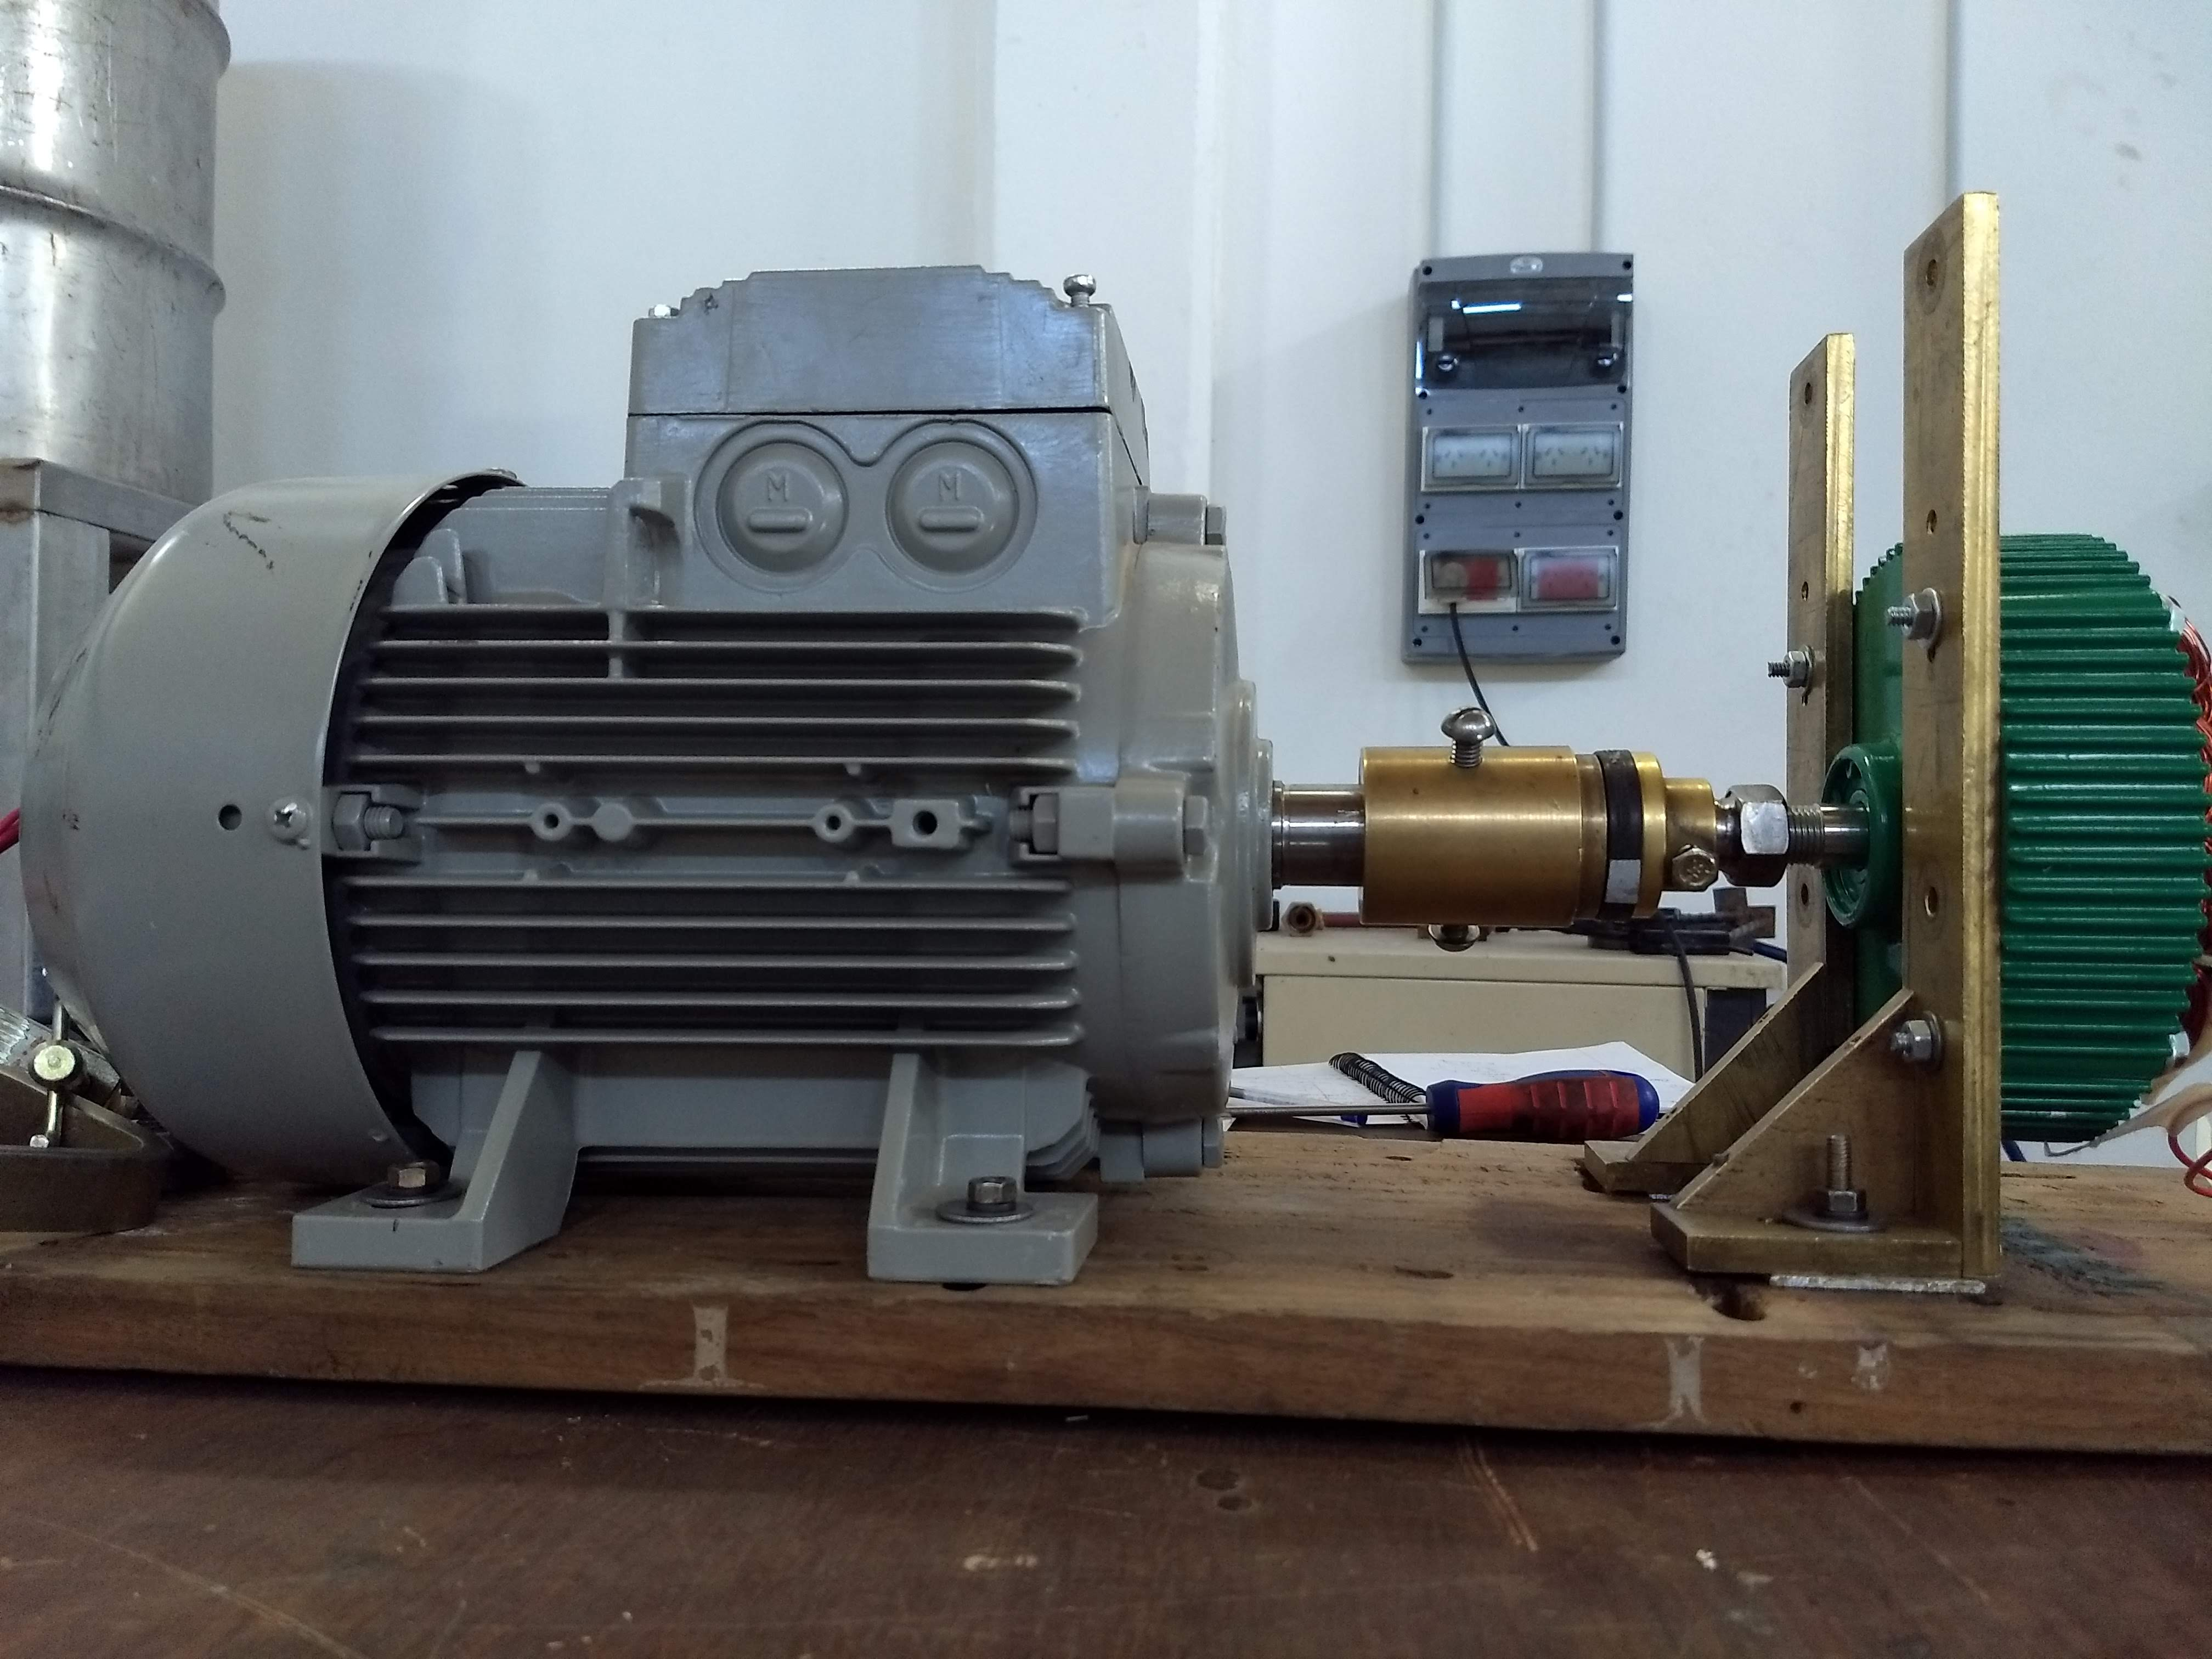
\includegraphics[width=0.45\textwidth]{Figuras/BancoProvisorioVistaLateral.jpg}}%
\hfill % <-- Seperation
\subcaptionbox{Vista superior}{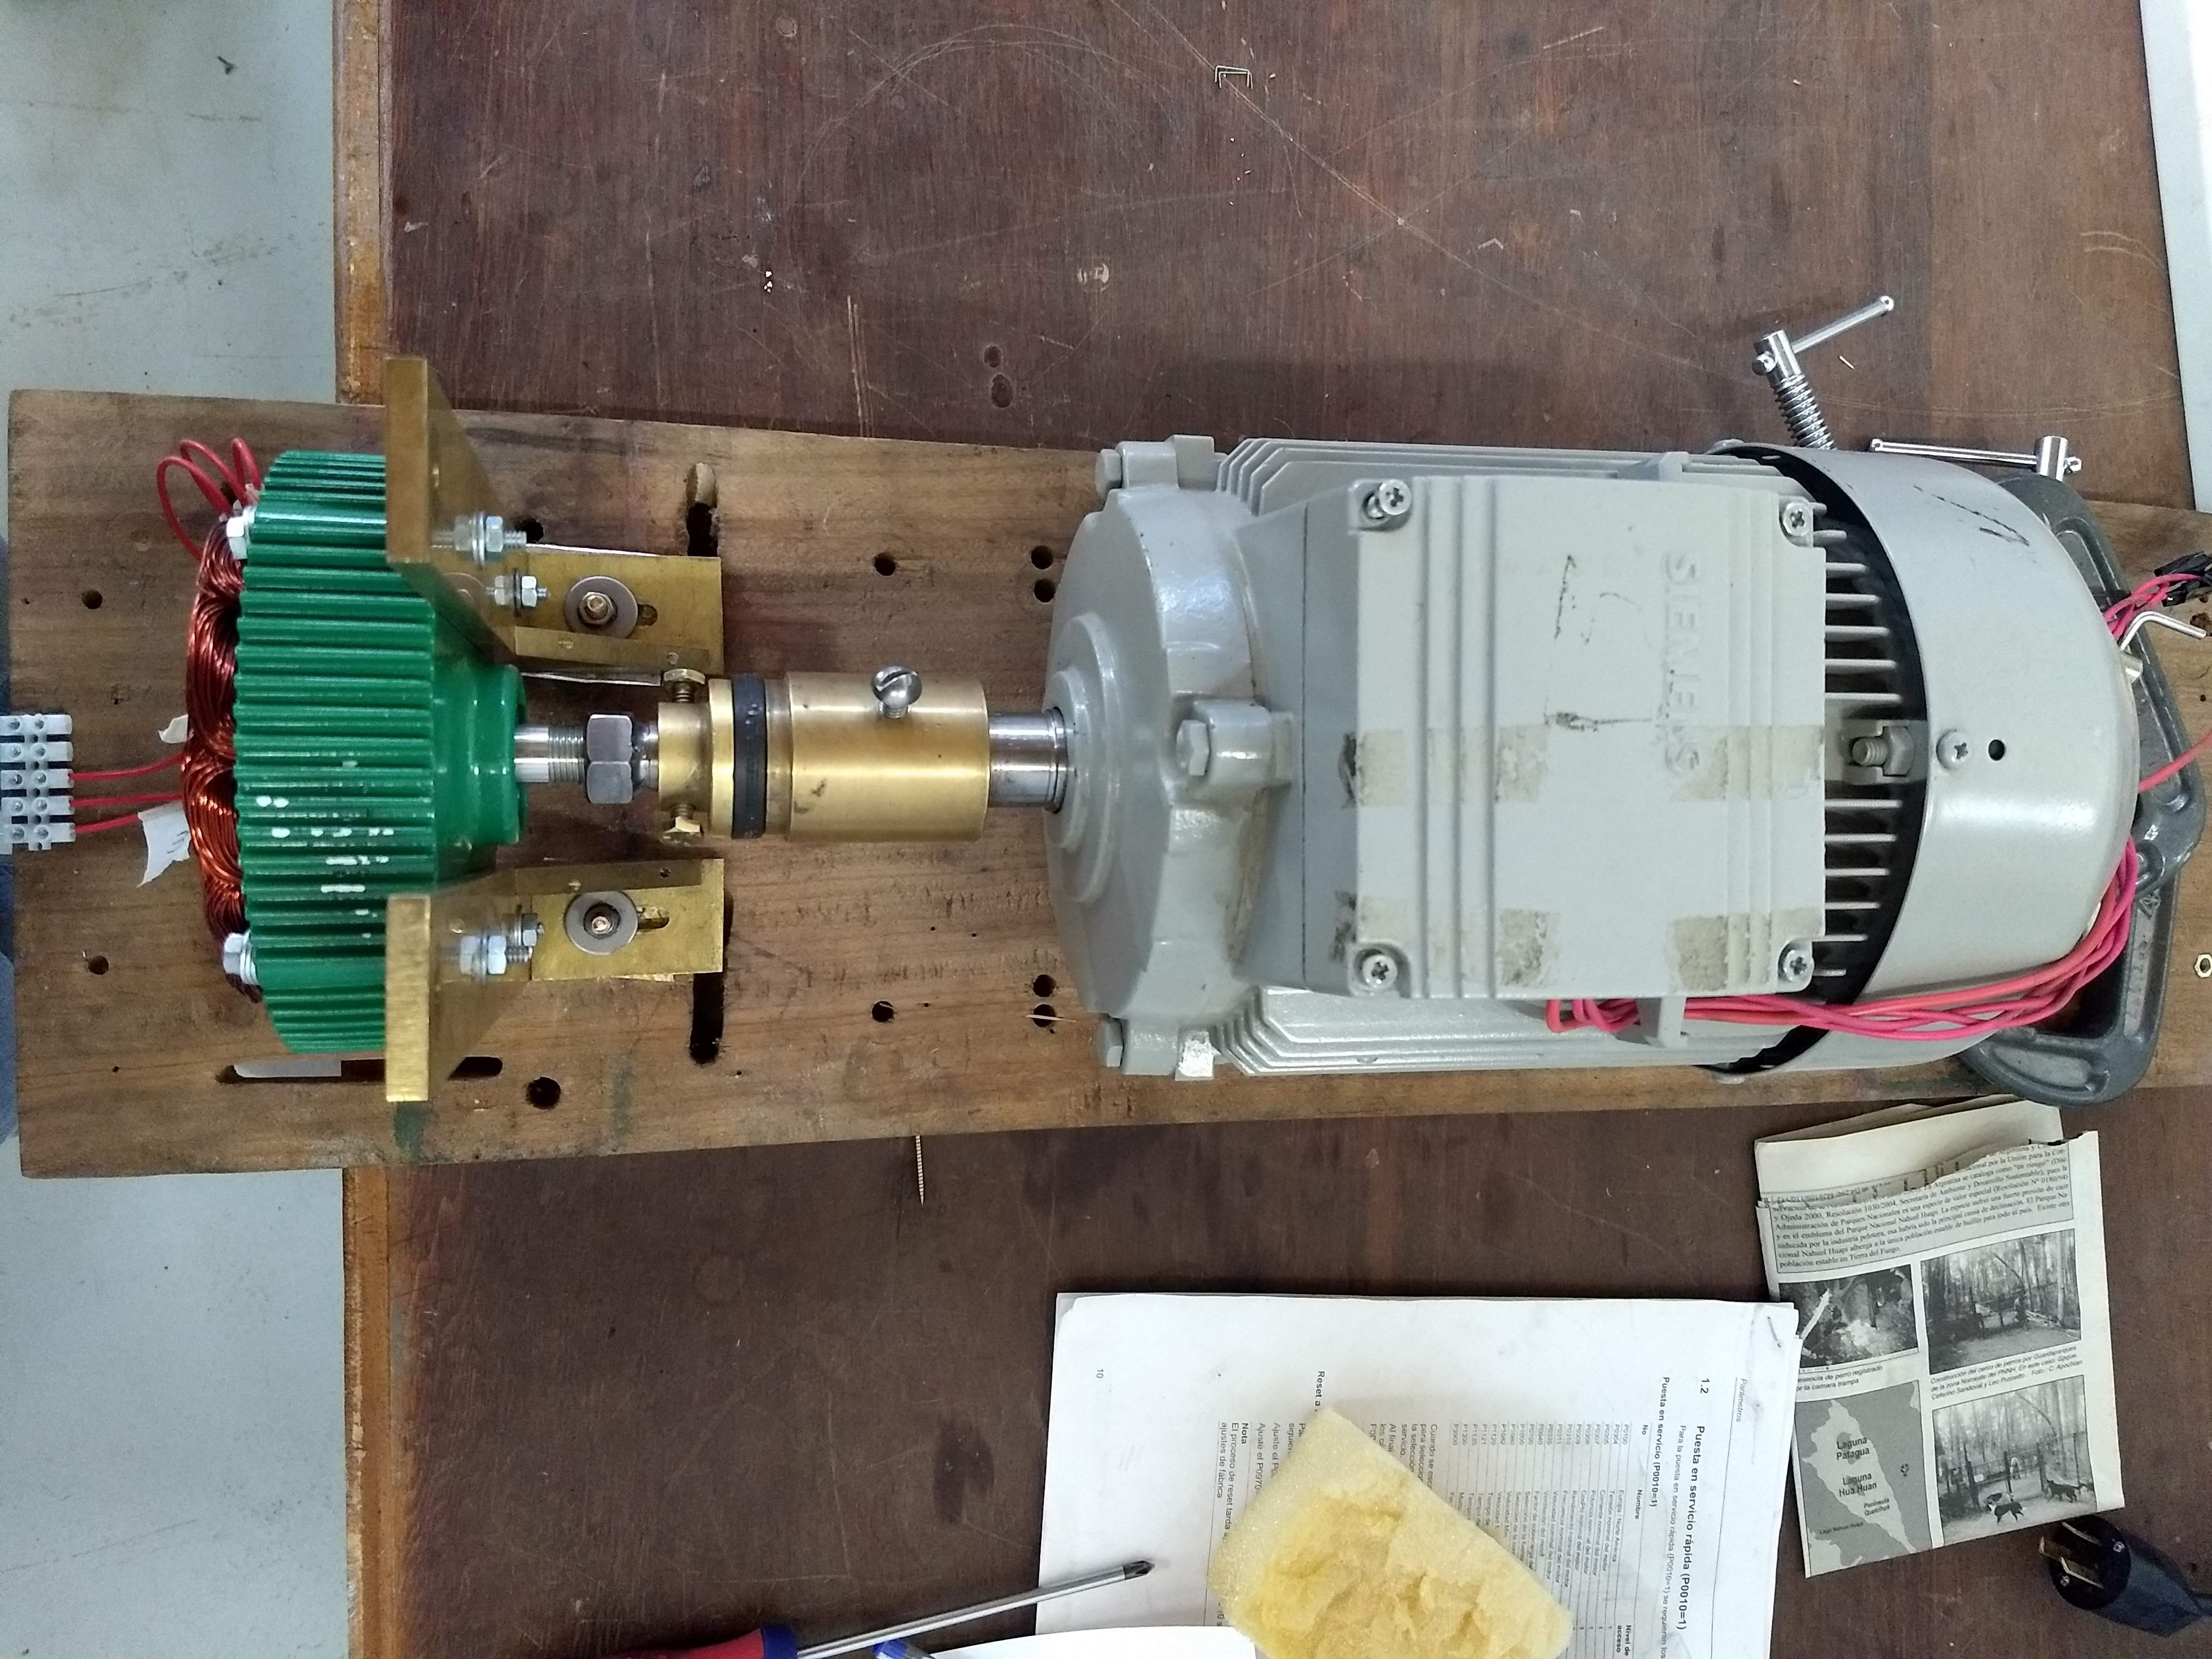
\includegraphics[width=0.45\textwidth]{Figuras/BancoProvisorioVistaSuperior.jpg}}%
\caption{Banco de ensayos provisorio}
\label{fig:bancoEnsayoVistas}
\end{figure}
\par Con el banco construido sólo restaba comenzar los ensayos característicos de vacío y en carga. Previamente se consultaron \cite{generador1}, \cite{generador2} y \cite{generador3}, trabajos donde la cátedra ya había trabajado en la caracterización de generadores. En estos, conocí que instrumental disponible del Laboratorio de Ingeniería se utilizó y debía entonces hacer uso para la caracterización del presente generador.
\par En los ensayos de vacío se varío la frecuencia del variador entre 5 y 20 $Hz$ para así variar las $RPM$. Estas se midieron con un tacómetro digital. La tensión en bornes del generador se midió tanto con un osciloscopio analógico como con multímetros digitales de distintas precisiones. Mediante el osciloscopio, se pudo determinar que la onda generada tiene forma sinusoidal con algunas deformaciones, y que por lo tanto el valor eficaz registrado mediante un multímetro es congruente con la tensión en bornes. 
\\ Para poder medir con el osciloscopio debió implementarse un divisor resistivo que atenuará la tensión del generador. Esto se debió a que cuando se utiliza el variador de frecuencia en el rango de 10 a 20 $Hz$, la tensión pico a pico generada excede el rango de entrada de tensión del osciloscopio.
\\ En la figura Nº\ref{fig:OsciloscopioVacio} se muestra la fotografía de una medición en vacío con el variador de frecuencia a 10 $Hz$, correspondiente a $600\,RPM$. La escala del tensión se encuentra en $5\,VOLTS/DIV$, por lo que se tienen entre 35 y 40 $V_{p-p}$. Y la escala temporal se encuentra en $5\,ms/DIV$, contando aproximadamente $3.6$ divisiones se tiene un período de $18\,ms$ (y por lo tanto una frecuencia de $56\,Hz$). Asimismo, en la figura se aprecia la forma sinusoidal de la onda generada. 
\begin{figure}[h!]
\centering
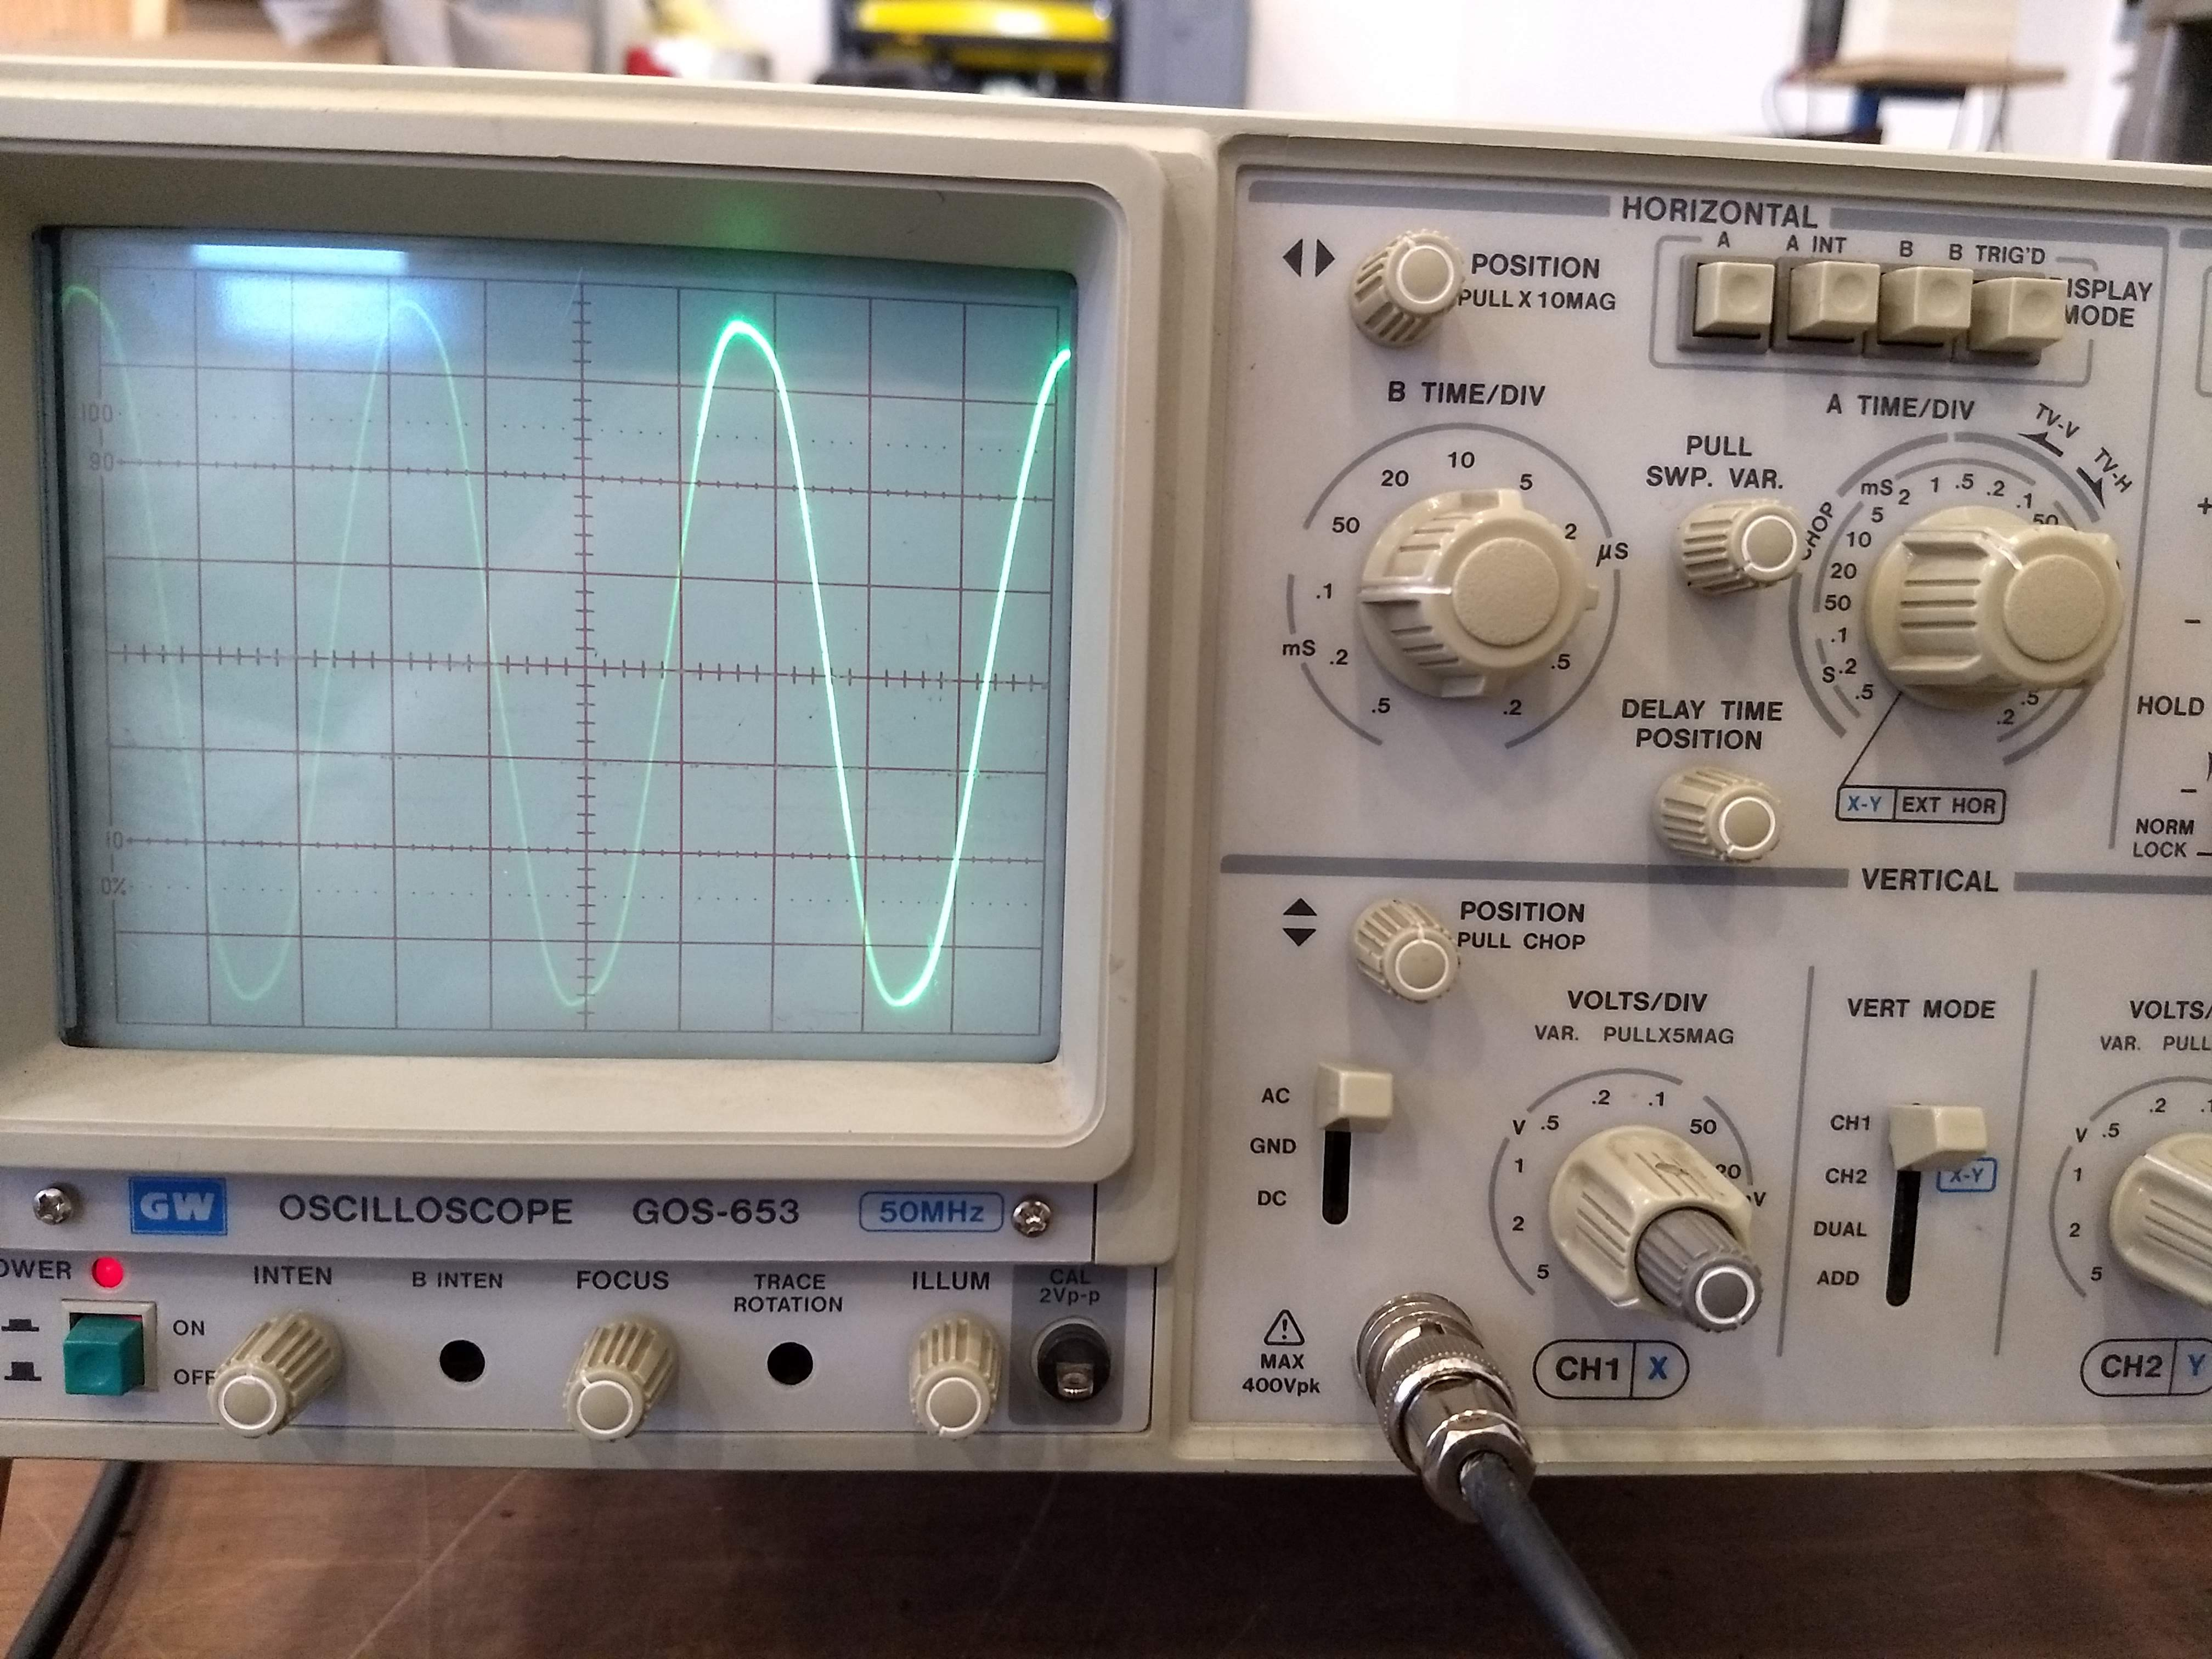
\includegraphics[width=8cm]{Figuras/OsciloscopioVacio.jpg}
\caption{Medición en vacío. Frecuencia del variador: $10\,Hz$. Notar la forma sinusoidal de la onda generada.}
\label{fig:OsciloscopioVacio}
\end{figure}
\par Luego, se realizaron los ensayos en carga del generador. Previamente se hicieron cálculos para tener idea de la corriente máxima que se podía tener por fase. Como carga, se utilizó un reóstato de $750\,W$ y $5\,\varOmega$ de resistencia máxima en serie con una resistencia pratrón (shunt) de $1\,\varOmega$. Utilizando dos multímetros digitales se medía la tensión en bornes del generador y en bornes del patrón. Cabe mencionar que no fue posible cargar las tres fases por igual (ya sea en estrella o triángulo), por lo que la carga se conectó entre dos fases. 
\\En la figura Nº\ref{fig:EnsayoCarga} se muestra el montaje realizado para el ensayo en carga. El osciloscopio se conectó eventualmente para verificar que la forma de onda continuara siendo sinusoidal.
\begin{figure}[h!]
\centering
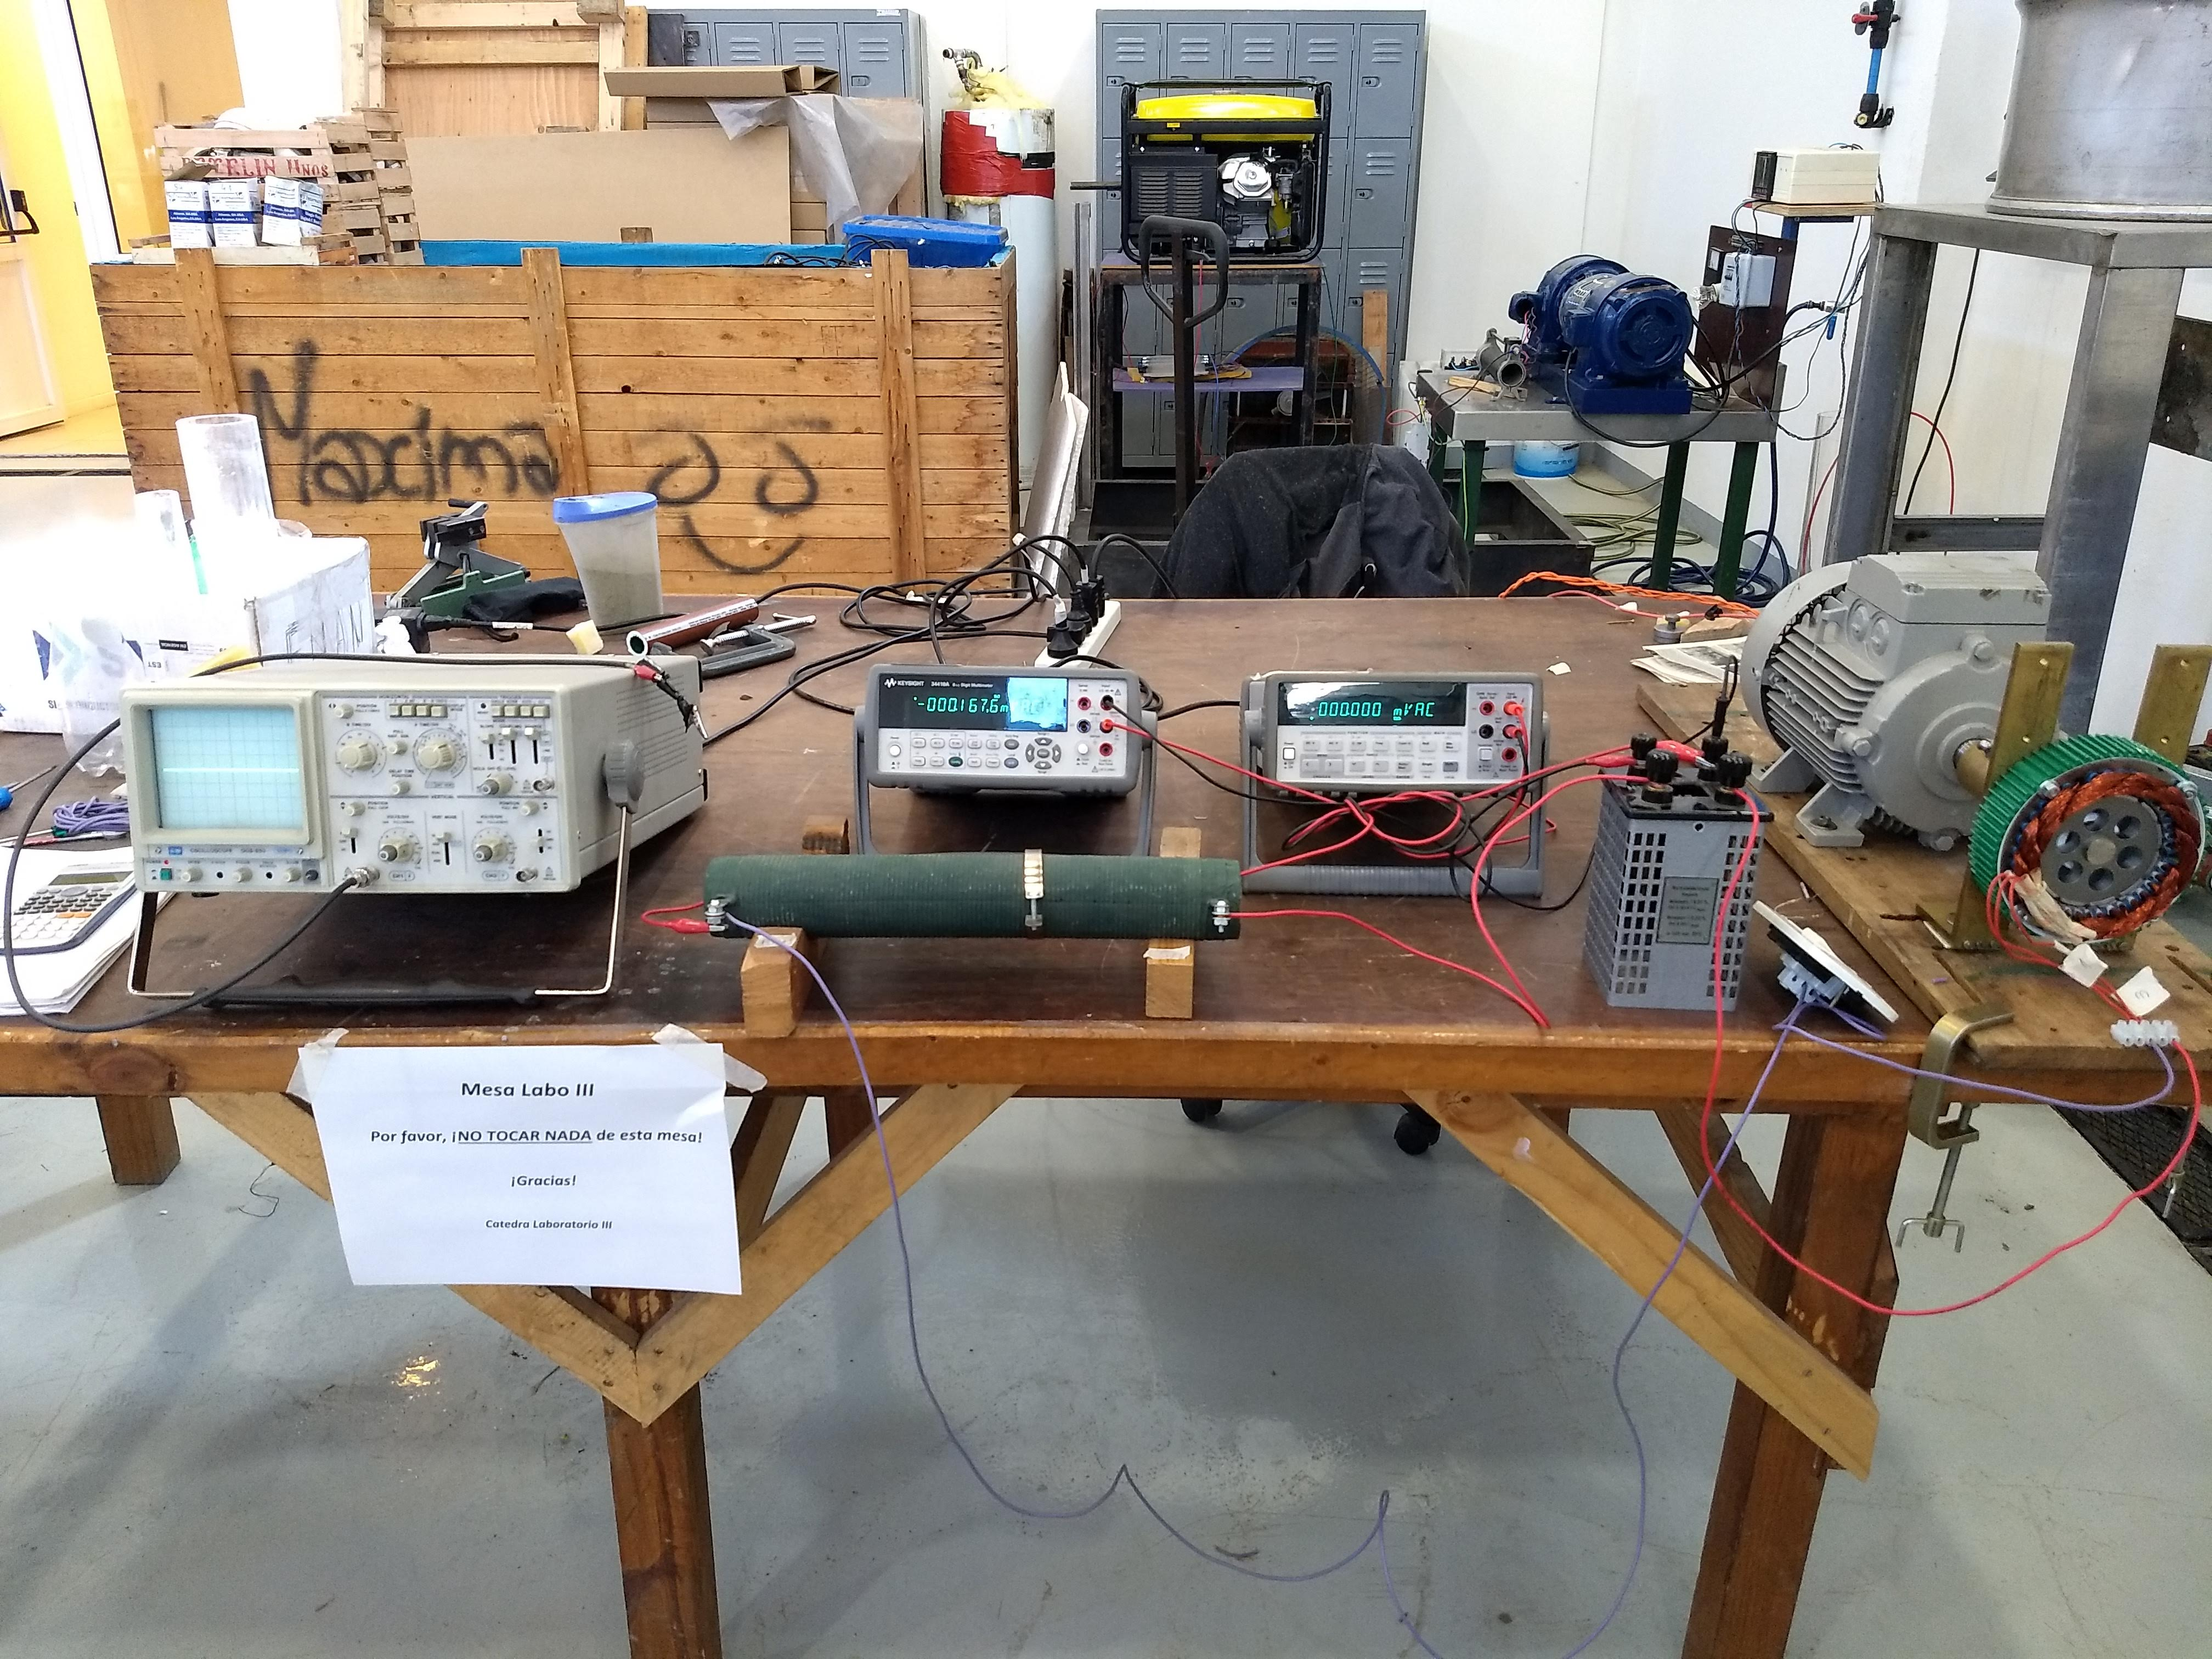
\includegraphics[width=8cm]{Figuras/EnsayoCarga.jpg}
\caption{Montaje para el ensayo en carga.}
\label{fig:EnsayoCarga}
\end{figure}
\par Finalmente, para realizar el ensayo en cortocircuito se desconectó el reóstato y se reemplazó el patrón de $1\,\varOmega$ por uno de $0.01\,\varOmega$. Si bien esto no representa idealmente un cortocircuito, la resistencia del patrón resulta del orden de más de cien veces menor que la del bobinado del generador.
\\Un parámetro que cobró importancia en los ensayos en carga y en cortocircuito fue la temperatura. A medida que la corriente que circula aumenta, también lo hace la temperatura de reóstato y del bobinado, disminuyendo la resistencia y por lo tanto aumentando la corriente y disminuyendo la tensión generada. 
\newpage
\section{MEMORIA TÉCNICA}
\subsection{Medición de los bobinados}
Para la medición de los bobinados se utilizó el analizador de impedancia \textit{Agilent E4980A - Precision LCR Meter}, que permite un barrido en frecuencia de 20 $Hz$ a 2 $MHz$. Como se mencionó en la Memoria Descriptiva, dada la sofisticación del equipo, primero se me explicó su principio de funcionamiento y como emplearlo. Para esto último, se midieron resistencias, capacitores y solenoides a distintas frecuencias. Estas mediciones se realizaron a cuatro puntas (al igual que las posteriores de los bobinados).
\par Las mediciones de los bobinados se realizaron a tres frecuencias distintas: $20\,Hz$, $100\,Hz$ y $1000\,Hz$. Desafortunadamente, la frecuencia nominal de trabajo del generador de $15\,Hz$ ($900\,RPM$) resulta fuera del rango del analizador. En las tablas Nº\ref{tabla:bobinas1-2}, Nº\ref{tabla:bobinas2-3} y Nº\ref{tabla:bobinas1-3} se muestran los resultados de las mediciones. Los valores de inductancias y de resistencia corresponden a la configuración del analizador donde muestra estos dos como el equivalente de un circuito serie. 
\begin{table}[h!]
\centering
\caption{Mediciones terminales 1-2}
\label{tabla:bobinas1-2}
\begin{tabular}{|c|c|c|c|c|}
\hline
Frecuencia $Hz$ & Inductancia $mH$ & Resistencia $\varOmega$ & Impedancia $\varOmega$ & Ángulo de fase º \\ \hline 
$20$&$9.6$&$1.7$&$2.1$&$35$  \\ \hline
$100$&$1.45$&$1.132$&$1.45$&$38.8$  \\ \hline
$1000$&$1.8333$&$1.383$&$11.6$&$83.01$  \\ \hline
% $$&$$&$$&$$&$$  \\ \hline
\end{tabular}
\end{table}
\begin{table}[h!]
\centering
\caption{Mediciones terminales 2-3}
\label{tabla:bobinas2-3}
\begin{tabular}{|c|c|c|c|c|}
\hline
Frecuencia $Hz$ & Inductancia $mH$ & Resistencia $\varOmega$ & Impedancia $\varOmega$ & Ángulo de fase º \\ \hline 
$20$&$2.4$&$1.2$&$1.25$&$13.8$  \\ \hline
$100$&$1.44$&$1.12$&$1.44$&$38.9$  \\ \hline
$1000$&$1.5234$&$1.316$&$9.662$&$82.16$  \\ \hline
% $$&$$&$$&$$&$$  \\ \hline
\end{tabular}
\end{table}
\begin{table}[h!]
\centering
\caption{Mediciones terminales 1-3}
\label{tabla:bobinas1-3}
\begin{tabular}{|c|c|c|c|c|}
\hline
Frecuencia $Hz$ & Inductancia $mH$ & Resistencia $\varOmega$ & Impedancia $\varOmega$ & Ángulo de fase º \\ \hline 
$20$&$3.2$&$1.2$&$1.26$&$18.3$  \\ \hline
$100$&$1.59$&$1.12$&$1.5$&$41.6$  \\ \hline
$1000$&$1.686$&$1.35$&$10.68$&$82.75$  \\ \hline
% $$&$$&$$&$$&$$  \\ \hline
\end{tabular}
\end{table}
\par A partir de estas mediciones se puede realizar un circuito equivalente entre cada par de terminales. Si bien lo óptimo sería tener el circuito equivalente por fase, se desconoce si las bobinas están conectadas en estrella o triángulo pues estas conexiones están ocultas y sólo se tiene acceso a los terminales. 
\\ Observando, el ángulo de fase se puede apreciar como al aumentar la frecuencia el circuito se vuelve altamente inductivo puesto que la reactancia inductiva es proporcional a la frecuencia. De todas maneras, el generador no operará a altas frecuencias. También, se puede apreciar que la resistencia varía aproximadamente un 11\% respecto de su máximo (cuando en el ideal debería ser constante). 
\subsection{Factibilidad de uso del motor de CC}
Como se mencionó anteriormente, el motor provenía de una máquina caminadora y no se tenían más datos. Es decir, no se contaba con la chapa con las características del motor. y desafortunadamente en internet tampoco se encontró más información que este tipo de motores operan con una tensión del rango de $100V_{cc}$
Por lo tanto, había que ponerlo en marcha y realizar algunas pruebas que dieran idea de la potencia que era capaz de desarrollar. 
\par En primera instancia se lo conectó a una fuente de CC de $0-60\,V$ y $0-30\,A$, marca \textit{RAFE S.A}. Como es natural, al variar la tensión de la fuente, varía la velocidad del giro el motor. Sin embargo, al variar el potenciómetro de la tensión, el voltímetro no respondía acorde al cambio, si no que ''se demoraba". Esto se debe a que la carga inductiva del motor era significante para la fuente, por lo que decidió cambiar de fuente.
\\La nueva fuente conectada fue una de $0-40\,V$ y $0-10\,A$, de la marca \textit{HP}. Esta ya no sufría el inconveniente de la anterior al variar la tensión. Alimentando el motor con $40\,V$ se obtuvieron $1235\,RPM$ en vacío. Luego, tratando de simular un ensayo de rotor bloqueado, se frenaba el eje con la zuela de la zapatilla y se llegó a registrar una corriente de alrededor de $6\,A$ (con la tensión constante a $40\,V$). Con esta prueba rápida, se tiene  idea de que el motor desarrolla aproximadamente $240\,W$.
\par Si bien la potencia obtenida del motor es aproximada, es información suficiente para determinar que este motor no posibilitará caracterizar completamente al generador. Es decir, se estaría limitando la caracterización hasta el límite de potencia del motor. Por lo tanto, se descarta el uso de este motor de corriente continua y se opta por utilizar un motor asíncrono trifásico de 3 $kW$ disponible en el Laboratorio de Ingeniería. 
\subsection{Acople entre el motor y el generador}
\subsubsection{Banco de ensayos}
Definido el motor, se continuó con el acople entre este y el generador. Como se acaba de mencionar, el motor es propiedad del Labotorio de Ingeniería por lo que el banco construido es provisorio durante el transcurso de la materia. Este, es sencillamente una tabla de madera a la cual se han fijado el motor y el generador (ver figura Nº\ref{fig:bancoEnsayoVistas}). Este último se fijó a través de dos soportes de bronce. 
\\Para acoplar los ejes entre sí se utilizaron manchones de bronce vinculados mediante un acople elástico. Previamente, la ubicación del generador en los soportes de bronce se determinó de manera tal que los centros de eje estuvieran lo más alineados posibles para que el acople elástico absorba la menor desalineación posible. 
\\A priori, sujeta uno de los manchones al eje del generado resultó en una problemática puesto este se encuentra roscado ya que es donde apreta la tuerca que sujeta las hélices. La solución fue utilizar una tuerca que rosque en el eje y en uno de sus extremos soldarle una trozo de eje cilindrico. Este trabajo realizado por Sebastián se muestra en la figura Nº\ref{fig:EjeGeneradorTuerca} (notar la prolijidad de la soldadura entre la tuerca y el trozo de eje). Cabe mencionar que el sentido de giro del motor quedó definido en el sentido de apriete de la tuerca. 
\begin{figure}[h!]
\centering
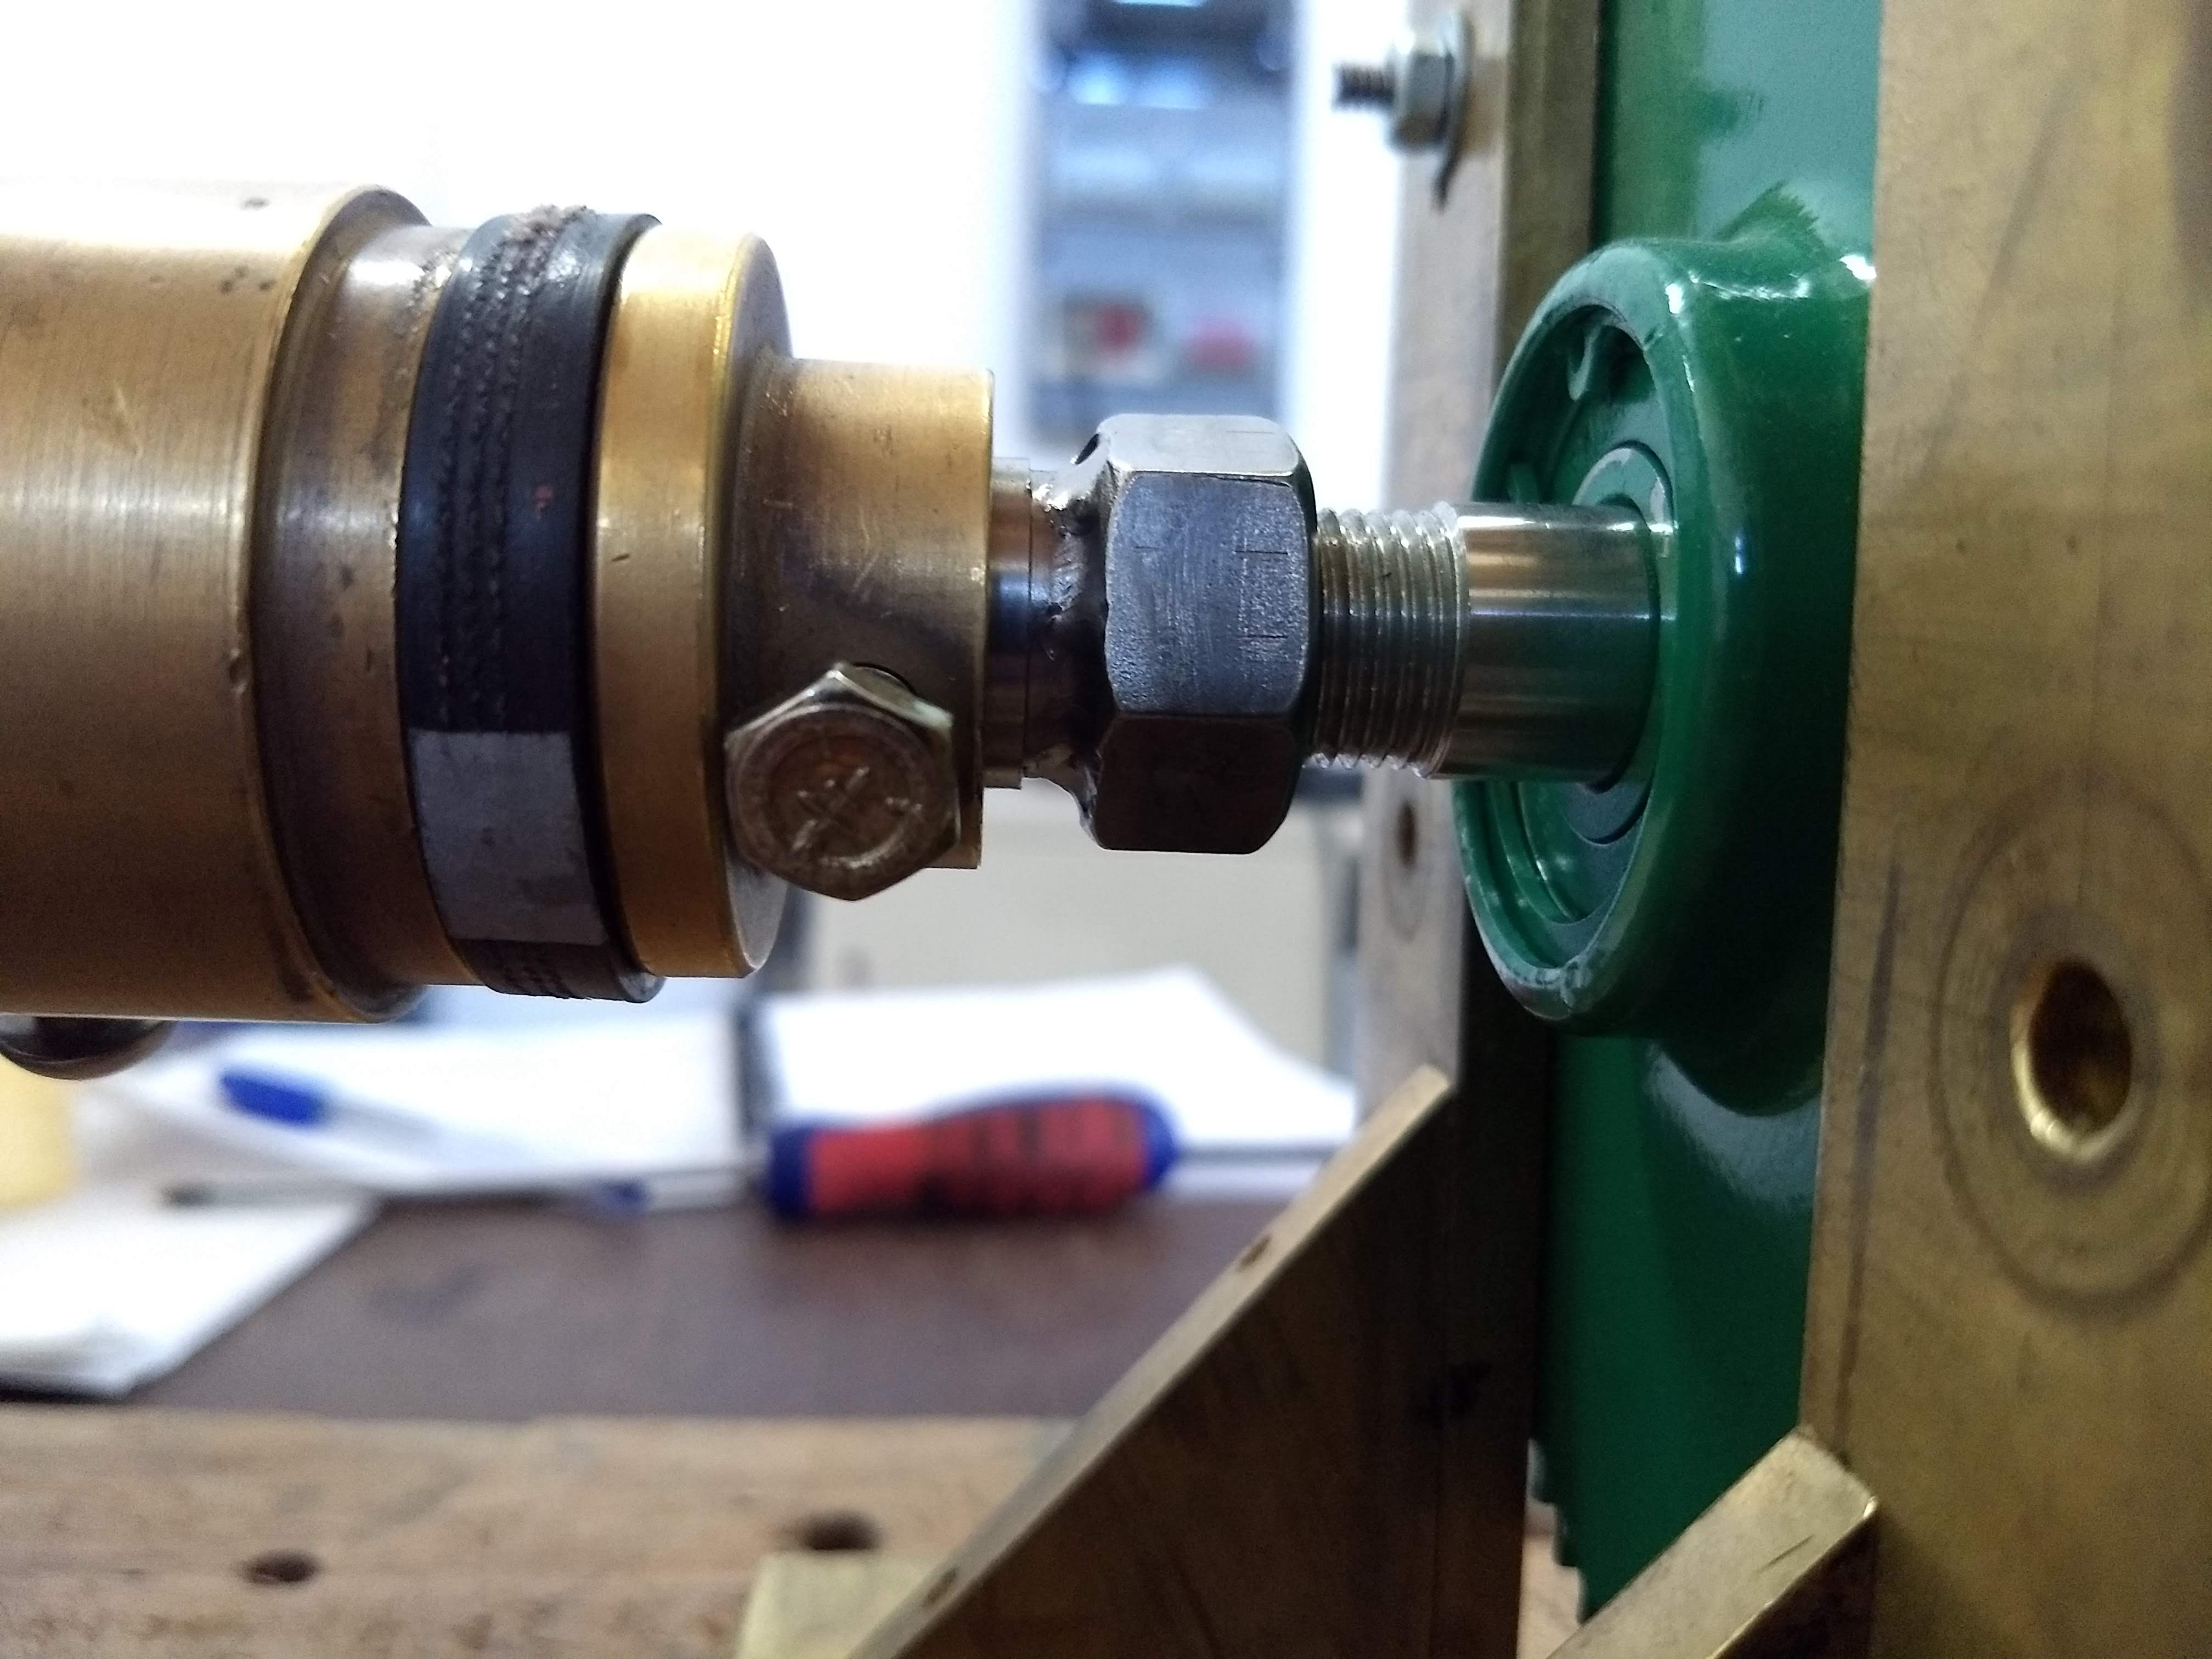
\includegraphics[width=8cm]{Figuras/EjeGeneradorTuerca.jpg}
\caption{Sujeción del manchón al eje del generador mediante una tuerca.}
\label{fig:EjeGeneradorTuerca}
\end{figure}
\subsubsection{Conexión del variador de frecuencia al motor}
El variador de frecuencia utilizado es un \textit{Siemens Sinamics G110 CPM 110 AIN} con las siguientes caracerísticas:
\begin{itemize}
\item Entrada
\begin{itemize}
\item $200-240\,V\pm10\%$ - Monofásico
\item $27.2\,A$
\item $47-63\,Hz$
\end{itemize}
\item Salida
\begin{itemize}
\item $0-230V$ - Trifásico
\item $11\,A$
\item Motor $2,2\,kW$ Duty Class II
\end{itemize}
\end{itemize}
Por su parte, las características del motor asíncrono trifásico son:
\begin{itemize}
\item $230/400\,V\,\varDelta/Y$
\item $10.6/6.1\,A\,\varDelta/Y$
\item $3kW$
\item $cos\phi = 0.85$
\item $2890\,RPM$
\end{itemize}
La información del motor es necesaria para configurar el variador. El rango de frecuencia de operación del variador se configuró desde 0 hasta 50 $Hz$, aunque siempre que se lo enciende comienza en $5\,Hz$.
\\Por último, el motor se conectó en triángulo y las fases se conectaron de manera tal que, como se mencionó anteriormente, el sentido de giro sea en el que apreta la tuerca. 
\subsection{Ensayos en vacío}
La primer medición se realizó encendiendo el variador a $5\,Hz$ y conectado entre dos de los terminales un multímetro digital, registrándose $18\,V$. Así se determinó que era seguro conectar el osciloscopio. Este se conecto en la máxima escala de tensión ($5\,VOLTS/DIV$) por precaución entre los terminales 1-3 y se pudo observar por primera vez que la onda generada esa sinusoidal.
\\Aumentando la frecuencia, al llegar a 10 $Hz$ el osciloscopio ya llega a su máximo rango máximo de tensión, por lo que para continuar midiendo con este iba a ser necesario implementar un divisor resistivo. Este, se pensó de manera tal que atenúe aproximadamente por 10 y que los valores de sus resistencia sean lo suficiente grande respecto a la resistencia del bobinado del generado y lo suficientemente pequeñas respecto de la impedancia de entrada del osciloscopio (comúnmente 10 $M\varOmega$ en los oscilocopios analógicos y 1 $M\varOmega$ en los digitales disponibles). De esta manera y entre las resistencias disponibles, se seleccionaron resistencias de 12 $k\varOmega$ y de 100 $k\varOmega$ (valores nominales) y se las conectó en serie. Luego, se las conectó entre dos terminales del generador y la el osciloscopio se mide la caída de tensión en la resistencia de 12 $k\varOmega$.
\\Las mediciones con el osciloscopio se realizaron variando la frecuencia del variador desde 5 $Hz$ hasta 20 $Hz$ con incrementos de 2.5 $Hz$. Hasta 10 $Hz$ inclusive se midió tanto con y sin el divisor, lo que permitió luego calcular el valor del divisor. Para las frecuencias superiores a 10 $Hz$ se utilizó el divisor.
\\Para calcular el valor del divisor, además de las tres mediciones del osciloscopio (con frecuencias a 5; $7.5$ y $10\,Hz$), se utilizaron multímetros digitales de diferentes exactitudes y preciones: el \textit{KEYSIGHT 34401A} y el \textit{MASTECH MY65}, el primero enormemente más sofisticado que el segundo. 
\begin{table}[h!]
\centering
\caption{Mediciones en vacío con el osciloscopio con y sin divisor resistivo}
\label{tabla:vacioOsc}
\begin{tabular}{|c|c|c|}
\hline
Frec. variador $Hz$ & Tension p-p sin divisor $V$& Tension p-p sin divisor $V$\\ \hline
$5$&$20$&$2K$ \\ \hline
$7.5$&$28$&$3K$ \\ \hline
$10$&$37$&$4K$ \\ \hline
$12.5$&$-$&$4.8K$ \\ \hline
$15$&$-$&$6K$ \\ \hline
$17.5$&$-$&$7K$ \\ \hline
$20$&$-$&$8K$ \\ \hline

%$$&$$ \\ \hline
\end{tabular}
\end{table}
\begin{table}[h!]
\centering
\caption{Exactitudes y precisiones de los multímetros utilizados para medir resistencia }
\label{tabla:multimetros}
\begin{tabular}{|c|c|c|c|}
\hline
Instrumento  & Exactitud $\varOmega$& Precisión $\varOmega$ & Observaciones\\ \hline 
KEYSIGHT 34401A &$0.002+0.001$& 1 &El fabricante especifica la exactitud como \\ 
& & & \% de lectura + \% de rango. Rangos\\ 
& & &de 100K y 10K\\ \hline
MASTECH MY65 & $\pm\,(0.5\%+3)$ & $10-1$ &10 en el rango de 200K y 1 en el de 20K\\ \hline
% $$&$$&$$&$$&$$  \\ \hline
\end{tabular}
\end{table}
\begin{table}[h!]
\centering
\caption{Mediciones con multímetro MASTECH MY-65 - Rango 200K}
\label{tabla:MASTECH200K}
\begin{tabular}{|c|c|}
\hline
R1 $k \varOmega$&R2 $k \varOmega$\\ \hline
$99.59$&$11.89$ \\ \hline
$99.55$&$11.89$ \\ \hline
$99.53$&$11.88$ \\ \hline
$99.55$&$11.88$ \\ \hline
$99.42$&$11.88$ \\ \hline
%$$&$$ \\ \hline
\end{tabular}
\end{table}
\begin{table}[h!]
\centering
\caption{Mediciones con multímetro ASTECH MY-65 - Rango 20K}
\label{tabla:MASTECH20K}
\begin{tabular}{|c|}
\hline
R2 $k \varOmega$\\ \hline
$11.890$ \\ \hline
$11.889$ \\ \hline
$11.891$ \\ \hline
$11.888$ \\ \hline
$11.890$ \\ \hline
%$$&$$ \\ \hline
\end{tabular}
\end{table}
\begin{table}[h!]
\centering
\caption{Mediciones con multímetro KEYSIGHT 34410A - Rangos 100K y 10K}
\label{tabla:KEYSIGHT100K}
\begin{tabular}{|c|c|}
\hline
R1 $k \varOmega$&R2 $k \varOmega$\\ \hline
$99.4$&$11.875$ \\ \hline
$99.4$&$11.865$ \\ \hline
$99.4$&$11.872$ \\ \hline
%$$&$$ \\ \hline
\end{tabular}
\end{table}
\par En la tabla Nº\ref{tabla:vacioOsc} se muestran la primer medición en vacío realizada. Como todavía no se conoce el valor de la constante \textit{K} asociada al divisor resistivo, cada lectura se registró como $XK$.
\\En las tablas Nº\ref{tabla:MASTECH200K}, Nº\ref{tabla:MASTECH20K} y Nº\ref{tabla:KEYSIGHT100K} se encuentran las mediciones realizadas con los multímetros para también determinar el valor de \textit{K}. Este resultó:
\begin{table}[h!]
\centering
\caption{Determinación constante del divisor rsistivo \textit{K}}
\label{tabla:determinacionK}
\begin{tabular}{|c|c|c|c|}
\hline
Instrumento  & K & $\pm \delta K$ & Observaciones\\ \hline 
KEYSIGHT 34401A &$9.3736$&$0.00209$&Rangos 100K y 10K \\ \hline
MASTECH MY65 & $9.375$ & $0.05932$ &Rango 200K\\ \hline
MASTECH MY65 & $9.371$ & $0.05927$ &Rangos 200K y 20K\\ \hline
Osciloscopio& $9.3793$ & - & - \\ \hline
% $$&$$&$$&$$&$$  \\ \hline
\end{tabular}
\end{table}
\par En el caso del cálculo de \textit{K} mediante las mediciones el osciloscopio, no se tiene el valor de la desviación pues el valor de \textit{K} corresponde a una regresión lineal sin ordenada al origen, y \cite{taylor} explica como calcular la desviación cuando la regresión es de la forma $y=mx+b$.
\\De la tabla Nº\ref{tabla:determinacionK} se adopta que el valor de K que se utilizará es $K=9.37$, despreciando a partir de la centésima.
\par Determinado el valor de \textit{K}, se realizaron nuevas mediciones de RPM mediante un tacómetro digital y del período de la onda generada mediante el osciloscopio. También se midió nuevamente la tensión de generación mediante el osciloscopio. Estas mediciones se muestran en la tabla Nº\ref{tabla:vacio} y partir de estas se realizan las gráficas de las figuras Nº\ref{fig:Vacio-TensionPP}, Nº\ref{fig:VacioTensionEf} y Nº\ref{fig:VacioFrecuencia}.
\begin{table}[h!]
\centering
\caption{Ensayo en vacío: terminales 1-3}
\label{tabla:vacio}
\begin{tabular}{|c|c|c|c|}
\hline
Frec. var. $Hz$ & \textit{RPM} & Período $ms$ & Tensión pico a pico $V$\\ \hline

$5$&$299$&$33$&$18$ \\ \hline
$7.5$&$450$&$22$&$27$ \\ \hline
$10$&$600$&$17.6$&$35$ \\ \hline
$12.5$&$751$&$13.6$&$46.87\,(5K)$ \\ \hline
$15$&$900$&$11.2$&$56.24\,(6K)$ \\ \hline
$17.5$&$1051$&$9.6$&$65.62\,(7K)$ \\ \hline
$20$&$1200$&$8.4$&$74.99\,(8K)$ \\ \hline
\end{tabular}
\end{table}
\begin{figure}[h!]
\centering
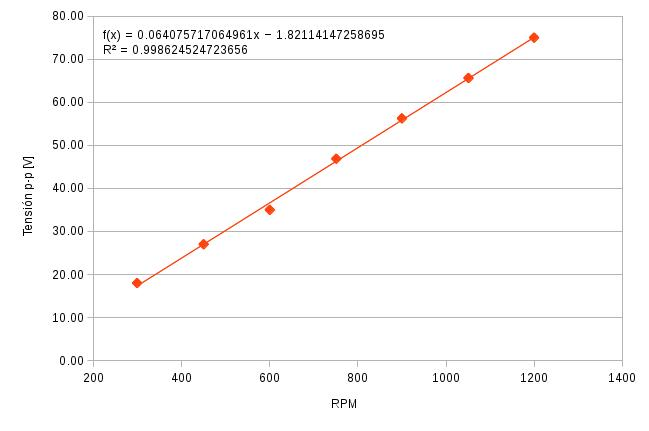
\includegraphics[width=8cm]{Figuras/Vacio-TensionPP.jpg}
\caption{Ensayo en vacío: tensión p-p vs. RPM}
\label{fig:Vacio-TensionPP}
\end{figure}
\begin{figure}[h!]
\centering
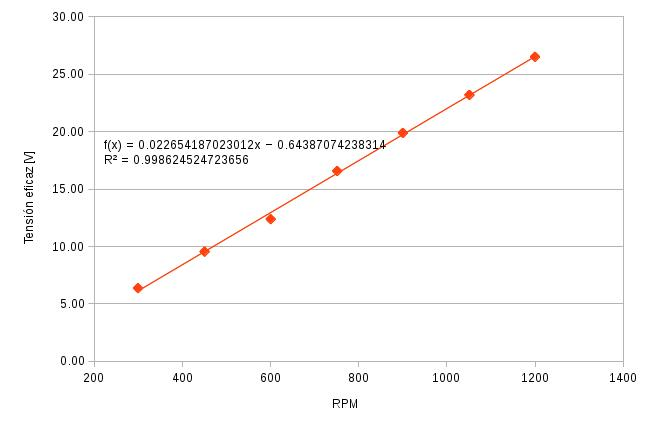
\includegraphics[width=8cm]{Figuras/VacioTensionEf.jpg}
\caption{Ensayo en vacío: tensión eficaz calculada a partir de la tensión p-p vs. RPM}
\label{fig:VacioTensionEf}
\end{figure}
\begin{figure}[h!]
\centering
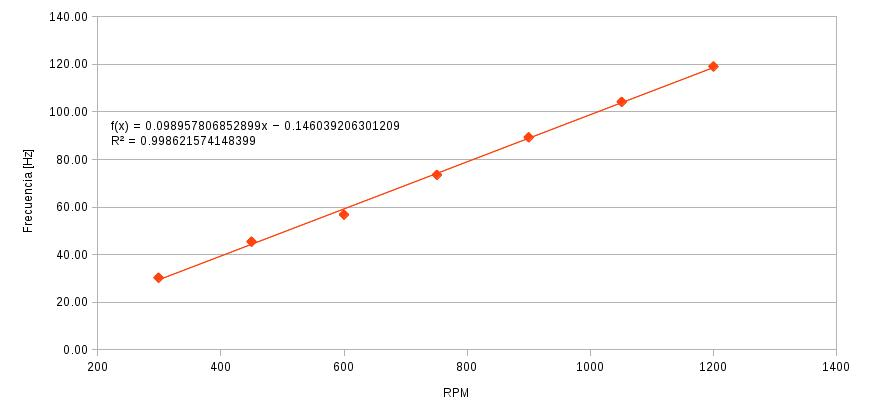
\includegraphics[width=8cm]{Figuras/VacioFrecuencia.jpg}
\caption{Ensayo en vacío: Frecuencia de la onda generada vs. RPM}
\label{fig:VacioFrecuencia}
\end{figure}
\subsection{Ensayos en carga}
Como se mencionó en la Memoria Descriptiva, el ensayo de carga se realizó conectando un reóstato de $750\,W$ y 5 $\varOmega$ de resistencia máxima en serie con una resistencia patrón de $1\,\varOmega\pm0.03\%$, de 3 $A$ de corriente máxima admisible. Si bien se cuenta con otra resistencia patrón que admite hasta 30 \textit{A}, esta es de $0.01\varOmega\pm 0.03\%$. Para una dada corriente, en este último patrón la caída de tensión es 100 veces menor que en el primero, resultando en una lectura mucho más pequeña y susceptible al ruido. Por esta razón, para esta instancia se decidió utilizar el patrón de $1\varOmega$.
\\Para medir la tensión en bornes del generador se utilizó el multímetro \textit{KEYSIGHT 34401A} y para medir la caída de tensión en el patrón el multímetro \textit{AGILENT 34401A}. También se contó con el osciloscopio para verificar si la forma de onda se veía afectada con el generador en carga, el tacómetro digital para relevar las \textit{RPM} y un multímetro digital \textit{UT60E} para medir la temperatura de la bobina mediante una termocupla. 
A su vez, se conectó una llave de un punto para abrir el circuito rápidamente si fuese necesario.
\par Lo primero que se realizó fue encender el variador de frecuencia en 5 $Hz$ y se registró una tensión en el patrón de $0.885\,V$. Y dado que el patrón es de $1\varOmega$, la corriente resulta de $0.885\,A$. A partir de este punto, se aumentó la frecuencia para saber en que valor circulaban 3 \textit{A}, corriente máxima del patrón. Resultó ser a una frecuencia de $17.3\,Hz$. 
\\ Otra prueba previa que se realizó fue establecer la frecuencia del variador en 10 y 20 $Hz$ con el generador en vacío y conmutar a carga con la llave y registrar caída de tensión en el patrón. Luego, se repitió la medición pero comenzando con el generador en carga. Con esto, se pretendía ver si el comportamiento era distinto, pero las mediciones se repitieron.
\par En la tabla Nº\ref{tabla:carga645} se muestran las mediciones hechas con el reóstato en su máxima resistencia y en la tabla Nº\ref{tabla:carga319} utilizando el cursor del mismo. En cada caso, la resistencia total (reóstato + patrón) fue medida con el multímetro \textit{KEYSIGHT 34401A} previo a comenzar el ensayo.
\begin{table}[h!]
\centering
\caption{Ensayo en carga Nº1: resistencia total $6.45\,\varOmega$.}
\label{tabla:carga645}
\begin{tabular}{|c|c|c|c|}
\hline
Frec. var. $Hz$ & Tensión patrón $V$ & Tensión generación $V$  & \textit{RPM}\\ \hline

$5$&$0.885$&$5.564$&$298$ \\ \hline
$7.5$&$1.326$&$8.35$&$447$ \\ \hline
$10$&$1.762$&$11.097$&$596$ \\ \hline
$12.5$&$2.195$&$13.831$&$746$ \\ \hline
$15$&$2.624$&$16.535$&$896$ \\ \hline
$17.5$&$3.049$&$19.225$&$1046$ \\ \hline
$20$&$3.467$&$21.868$&$1195$ \\ \hline

\end{tabular}
\end{table}
\begin{figure}[h!]
\centering
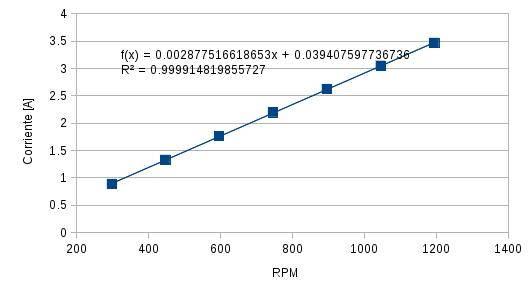
\includegraphics[width=8cm]{Figuras/CargaCorriente645.jpg}
\caption{Ensayo en carga total de $6.45\,\varOmega$: Corriente vs. RPM}
\label{fig:CargaCorriente645}
\end{figure}
\begin{figure}[h!]
\centering
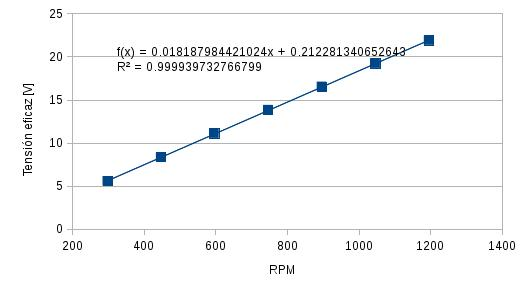
\includegraphics[width=8cm]{Figuras/CargaTension645.jpg}
\caption{Ensayo en carga de $6.45\,\varOmega$: Tensión eficaz vs. RPM}
\label{fig:CargaTension645}
\end{figure}
\begin{table}[h!]
\centering
\caption{Ensayo en carga Nº2: resistencia total $3.19\,\varOmega$.}
\label{tabla:carga319}
\begin{tabular}{|c|c|c|c|}
\hline
Frec. var. $Hz$ & Tensión patrón $V$ & Tensión generación $V$  & \textit{RPM}\\ \hline

$5$&$1.464$&$4.894$&$296$ \\ \hline
$7.5$&$2.195$&$7.307$&$445$ \\ \hline
$10$&$2.902$&$9.673$&$593$ \\ \hline
$12.5$&$3.598$&$11.941$&$745$ \\ \hline

\end{tabular}
\end{table}
\begin{figure}[h!]
\centering
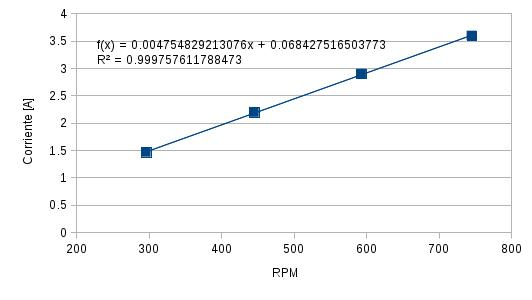
\includegraphics[width=8cm]{Figuras/CargaCorriente319.jpg}
\caption{Ensayo en carga de $3.19\,\varOmega$: Corriente vs. RPM}
\label{fig:CargaCorriente319}
\end{figure}
\begin{figure}[h!]
\centering
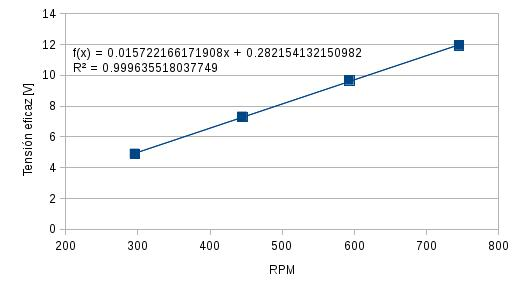
\includegraphics[width=8cm]{Figuras/CargaTension319.jpg}
\caption{Ensayo en carga de $3.19\,\varOmega$: Tensión eficaz vs. RPM}
\label{fig:CargaTension319}
\end{figure}
\par Nuevamente, dado que el patrón es de $1\,\varOmega$, la corriente resulta en magnitud igual a la caída de tensión en el patrón. En ambos ensayos se excedió el límite de corriente del patrón, por lo que las mediciones en esos puntos fueron muy breves. En este sentido, para el segundo ensayo se finalizó a $12.5\,Hz$.
\par Si bien se argumentó que el patrón de $0.01\,\varOmega$ sería más susceptible al ruido, en las mediciones hasta aquí realizadas se observó que este no era una molestia\footnote{Se debe destacar que el multímetro \textit{AGILENT 34401A} se configuró de manera tal minimizar la influencia del ruido.}. Esto motivo entonces a utilizar este patrón para realizar el ensayo en carga, arrojando las siguientes mediciones:
\begin{table}[h!]
\centering
\caption{Ensayo en carga Nº3: resistencia total $0.83\,\varOmega$.}
\label{tabla:carga083}
\begin{tabular}{|c|c|c|c|}
\hline
Frec. var. $Hz$ & Tensión patrón $V$ & Tensión generación $V$  & \textit{RPM}\\ \hline

$5$&$0.035$&$2.281$&$296$ \\ \hline
$7.5$&$0.050$&$3.320$&$442$ \\ \hline
$10$&$0.065$&$4.128$&$590$ \\ \hline
$12.5$&$0.076$&$4.800$&$738$ \\ \hline
$15$&$0.085$&$5.334$&$888$ \\ \hline
$17.5$&$0.093$&$5.858$&$1038$ \\ \hline
$20$&$0.100$&$6.300$&$1188$ \\ \hline

\end{tabular}
\end{table}
\begin{figure}[h!]
\centering
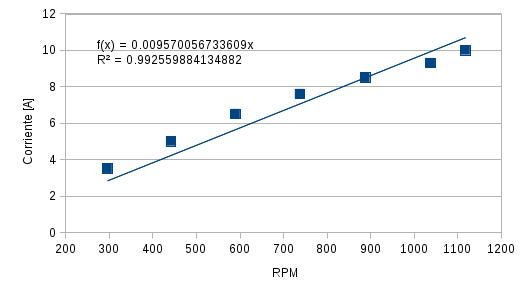
\includegraphics[width=8cm]{Figuras/CargaCorriente083.jpg}
\caption{Ensayo en carga de $0.83\,\varOmega$: Corriente vs. RPM}
\label{fig:CargaCorriente083}
\end{figure}
\begin{figure}[h!]
\centering
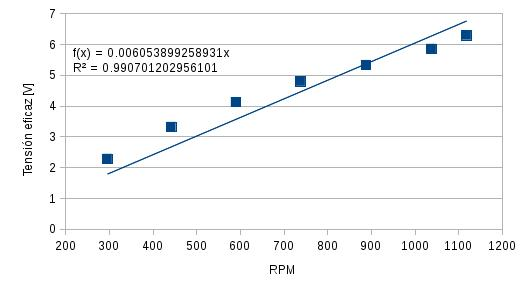
\includegraphics[width=8cm]{Figuras/CargaTension083.jpg}
\caption{Ensayo en carga de $0.83\,\varOmega$: Tensión eficaz vs. RPM}
\label{fig:CargaTension083}
\end{figure}
\par Ahora, la corriente es en magnitud 100 veces el valor de la caída de tensión en el patrón. En las mediciones se observa claramente como al disminuir la resistencia total aumenta la corriente para una frecuencia dada del variador de frecuencia. De hecho, se dificultó registrar la medición de la tensión de generación en el ensayo en carga Nº3 puesto que esta disminuía continuamente. Esto se deba a que al desarrollar corrientes tales como $9.3\,A$ y $10\,A$ la temperatura del bobinado comenzaba a aumentar significativamente cayendo entonces la tensión de generación. Las temperaturas alcanzas en estas últimas dos lecturas fueron 41ºC y 53ºC.
\subsection{Ensayo en cortocircuito}
Como se mencionó anteriormente, no se trata de un ensayo en cortocircuito ideal si no que de uno aproximado pues está conectado el patrón de $0.01\,\varOmega$. Considerando que las corriente sen juego iban a ser más significativas, no se registraron las RPM para no demorar las mediciones. Los resultados fueron:
\begin{table}[h!]
\centering
\caption{Ensayo cortocircuito}
\label{tabla:cortocircuito}
\begin{tabular}{|c|c|c|c|}
\hline
Frec. var. $Hz$ & Tensión patrón $V$ & Tensión generación $V$  & Temperatura ºC\\ \hline
$5$&$0.050$&$0.220$& - \\ \hline
$7.5$&$0.071$&$0.507$& - \\ \hline
$10$&$0.087$&$0.580$& - \\ \hline
$12.5$&$0.098$&$0.643$& - \\ \hline
$15$&$0.107$&$0.706$&$45$ \\ \hline
$17.5$&$0.113$&$0.709$&$50$ \\ \hline
$20$&$0.118$&$0.754$&$58$ \\ \hline

\end{tabular}
\end{table}
\begin{figure}[h!]
\centering
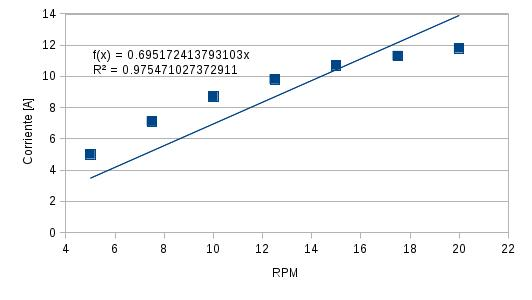
\includegraphics[width=8cm]{Figuras/CorrienteCortocircuito.jpg}
\caption{Ensayo de cortocircuito: Corriente vs. RPM}
\label{fig:CorrienteCortocircuito}
\end{figure}
\begin{figure}[h!]
\centering
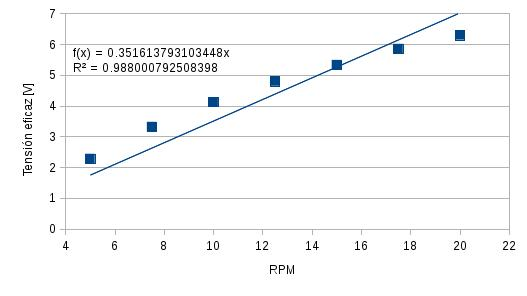
\includegraphics[width=8cm]{Figuras/TensionCortocircuito.jpg}
\caption{Ensayo de cortocircuito: Tensión eficaz vs. RPM}
\label{fig:TensionCortocircuito}
\end{figure}
\par Como bien se sabe, la circulación de corriente da lugar la denominada reacción de inducido que modifica el campo magnético de la máquina eléctrica. Para verificar si la forma de la onda de la generación se vió afectada, se conectó el osciloscopio. En la figura Nº\ref{fig:OsciloscopioCortocircuito} se muestra una fotografía del mismo, con la escala de tensión en $0.5\,VOLTS/DIV$ y la de tiempo en $5\,ms$. Como se puede observar, la onda continua siendo sinusoidal, con una tensión pico a pico de 2 $V$ (aproximadamente $0.707V_{ef}$) y un período de 8 $ms$ (equivalente a una frecuencia de 125 $Hz$).
\begin{figure}[h!]
\centering
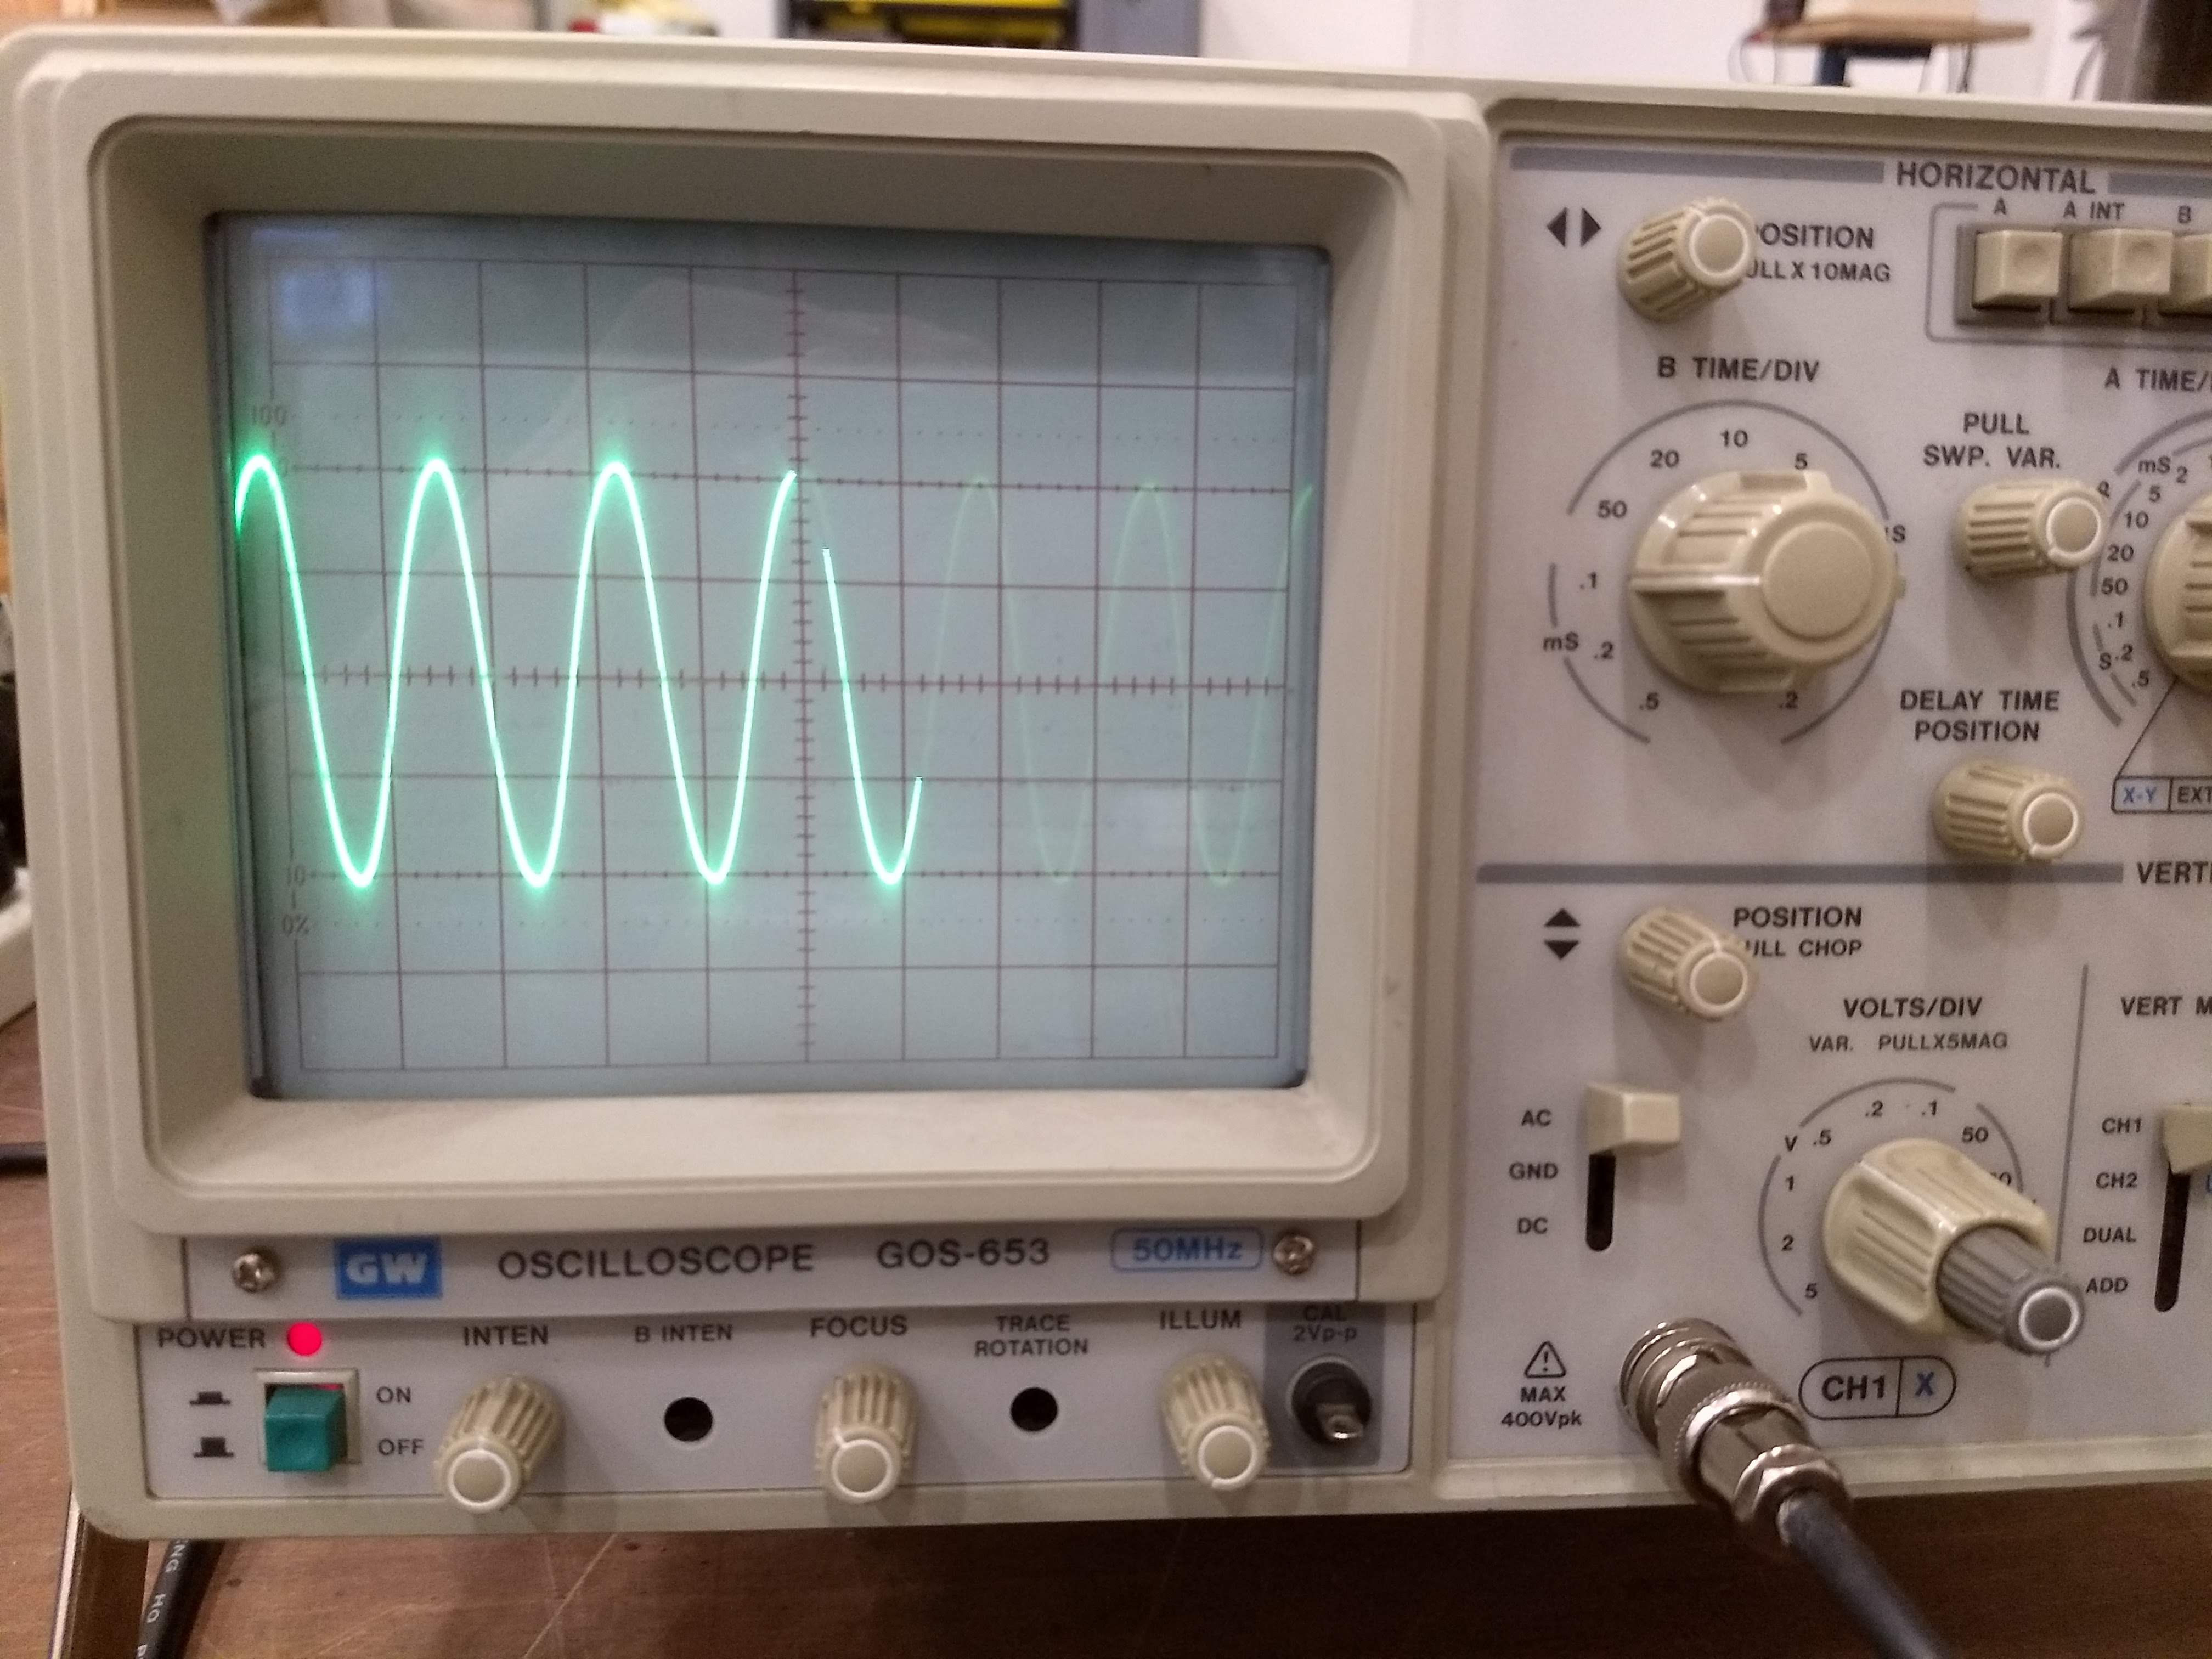
\includegraphics[width=8cm]{Figuras/OsciloscopioCortocircuito.jpg}
\caption{Verificación de la forma de onda en cortocircuito. Variador de frecuencia en 15 $Hz.$}
\label{fig:OsciloscopioCortocircuito}
\end{figure}
\section{Conclusiones}
El trabajo desarrollado en la materia hasta la fecha se relaciona directamente con el objetivo de la maestría. Si se pretende controlar la generación, es primordial contar con un modelo del generador. Por ello, todas las tareas de caracterización hechas hasta esta instancia resultan primordiales.
\\Como se mencionó anteriormente, al momento se desconoce si las bobinas del generador están conectados en estrella o triángulo. Claramente, esta revisión del conexionado es un trabajo a futuro y en función del ello sabrá como representarse el circuito equivalente del generador. La restante información se encuentra tanto en las mediciones de los bobinados como en los ensayos característicos realizados. 
\par En la primer ensayo en vacío resultó como una grata noticia que la forma de onda generada sea sinusoidal. Esto simplifica las mediciones puesto que da lugar a que se pueda medir la tensión eficaz haciendo uso de un multímetro digital. También, se verifica que la tensión generada y la frecuencia de la generación resultan lineales respecto de la velocidad de giro del motor. 
\par En los ensayos en carga también se observan algunos comportamiento característicos. Si se compara para una dada frecuencia del variador, al disminuir la carga, aumenta la corriente y cae la tensión generada. A su vez, en menor medida, se aprecia el deslizamiento. Y en el caso del tercer ensayo en carga, es notable el aumento de temperatura cuando circulan 10 \textit{A}.
\\ De hecho, este comportamiento nos hizo considerar lo siguiente. Si el generador es capaz de desarrollar una potencia de 400 $W$ a 900 $RPM$, en vacío corresponde a una tensión eficaz de aproximadamente $20\,V$ y por lo tanto una corriente por fase de $11.56\,A$. Esto daría lugar a un significativo aumento de la temperatura del bobina peligrando la vida útil del mismo. Si bien se trata de un aerogenerador y estaría montado al aire libre donde se favorecería la refrigeración, con la información disponible hasta aquí es dudoso que sea capaz de entregar 400 $W$ en régimen permanente. 
\par También en los ensayos en carga, las regresiones de los primeros dos ensayos muestran un comportamiento lineal, mientras que la del tercero no tanto. De hecho, se forzó el cruce por cero para obtener un mejor coeficiente de correlación. Este comportamiento empeora para el ensayo en cortocircuito, demostrando que tanto la corriente como la tensión no aumentan proporcionalmente a las RPM (o frecuencia del variador en caso del cortocircuito). Este comportamiento recuerda a la histéresis que sufre una máquina elétrica con excitación variable, pero este no es el caso. 
\par Otro aspecto de importancia en las diferentes mediciones realizadas a lo largo de este trabajo fue el estudio de incertezas. Por motivos de tiempo en la entrega de este informe no se lo ha desarrollado aquí como se lo merece, pero ha sido una tarea a la que nunca se dejo de lado. Y personalmente, durante este período fue donde más y mejor comprendí el análisis de incertezas.
\par Como trabajo futuro se tiene aún camino por realizar en el estudio del generador. Además de realizar los circuitos equivalentes, también resta por analizar la eficiencia de la generación por ejemplo. Para esto es necesario acoplar un torquímetro, y junto con la medición de las RPM se tendría la potencia mecánica que entra al generador. Luego, teniendo la potencia eléctrica se calcularía la eficiencia. 
\\También, en el caso que se considere por finalizada la caracterización del generador, puede avanzar con la caracterización del regulador de cargo y/o de las hélices. 
\end{document}
%que